\documentclass{article}

% Language setting
% Replace `english' with e.g. `spanish' to change the document language
\usepackage[english]{babel}
\usepackage{float}

% Set page size and margins
% Replace `letterpaper' with `a4paper' for UK/EU standard size
\usepackage[letterpaper,top=2cm,bottom=2cm,left=3cm,right=3cm,marginparwidth=1.75cm]{geometry}

% Useful packages
\usepackage{amsmath}
\usepackage{physics}
\usepackage{graphicx}
\usepackage{caption}
\usepackage{subcaption}
%\usepackage[style = numeric]{biblatex}
\usepackage[colorlinks=true, allcolors=blue]{hyperref}

%\title{Your Paper}
%\author{You}
%\addbibresource{trna.bib}
\begin{document}
\tableofcontents
\newpage
%\maketitle

%\begin{abstract}
%Your abstract.
%\end{abstract}

\section{Introduction}

To describe the evolution experiment, we proposed the mathematical model below based on the population of each type of bacterial strain. It is important to clarify that this models is a simplification and by no means it is assumed to be complete, in the sense that there can be additional mutations that are not yet included. Nonetheless, it is expressive enough to capture two big types of mutations which are relevant for the context of this experiment

\begin{subequations}\label{eqs:three_state_model}
\begin{align}
\dv{F}{t} &= \left( r_F\left(1 - \frac{\mu_{F\rightarrow D}}{\ln{2}} - \frac{\mu_{F\rightarrow S}}{\ln{2}}\right)F + r_D \frac{\mu_{D\rightarrow F}}{\ln{2}} D + r_S \frac{\mu_{S\rightarrow F}}{\ln{2}} S \right)\left(1-\frac{F + D + S}{K}\right)\\
\dv{D}{t} &=\left( r_F \frac{\mu_{F\rightarrow D}}{\ln{2}} F + r_D\left(1 - \frac{\mu_{D\rightarrow F}}{\ln{2}}\right)D \right) \left(1-\frac{F + D + S}{K}\right) \\
\dv{S}{t} &= \left( r_F \frac{\mu_{F\rightarrow S}}{\ln{2}} F + r_S\left(1 - \frac{\mu_{S\rightarrow F}}{\ln{2}}\right)S \right) \left(1-\frac{F + D + S}{K}\right) 
\end{align}
\end{subequations}
Where $F$ is the founder strain population, $D$ is the population of bacteria carrying a duplication, and $S$ is the population of bacteria with an additional stabilizing SNP mutation. The model parameters are the replication rates ($r_F, r_D, r_S$) mutation/loss rates ($\mu_{F\rightarrow D}, \mu_{F\rightarrow S}, \mu_{D\rightarrow F}, \mu_{D\rightarrow S}$) and carrying capacity $K$. These equations assume that there is no direct transition between $D$ and $S$, and mutations can only happen upon replication. Additionally, the finite resources is introduced through the carrying capacity term in the equations.

An evolution experiment carried out through 100 days provides measurements of the fraction of large and small bacterial colonies at the end of every day. This data is used for the inference of the model's parameters. However, this inference task is not straightforward due to the inability of the experimental data to distinguish between the different types of mutations. 
Duplications and other mutations arise as a way to stabilize the genome after gene deletion, therefore it is plausible to assume that bacteria carrying mutations will have greater fitness and therefore they will be found in colonies of larger size. This consideration allow us to define a two state model that could be compared directly to the experimental data
The two state toy model is described by the following system of equations

\begin{subequations}\label{eqs:two_state_model}
\begin{align}
\dv{F}{t} &= \left( r_F\left(1 - \Tilde{\mu}_{FM}\right)F + r_M \Tilde{\mu_{MF}} M\right) \left(1-\frac{F + M}{K}\right)\\
\dv{M}{t} &= \left( r_F \Tilde{\mu_{FM}} F + r_M\left(1 - \Tilde{\mu}_{MF}\right)M\right) \left(1-\frac{F + M}{K}\right)
\end{align}
\end{subequations}
$F$, $M$ are the populations of founder and mutant strains, each with replication rate $r_F$, $r_M$ respectively. Mutations gain/loss occur with rate $\Tilde{\mu}_{FM} = \frac{\mu_{FM}}{\ln{2}}$, $\Tilde{\mu}_{MF} = \frac{\mu_{MF}}{\ln{2}}$.



It is important to note that even though Eqs \ref{eqs:three_state_model} and \ref{eqs:two_state_model} are used to describe the same phenomena, it is not possible to define an invertible linear transformation between the variables and parameters of both; therefore, it is necessary to search for an additional way to relate the set of parameters that could be determined independently for each model

To gain some understanding on the range of the model's parameters, we used values reported in [include reference] as well as parameters inferred from growth curves for individual strains which we detail below. The founder strain is referred to as \textit{delserCGA} and the reference mutant is \textit{M2lop}

\begin{table}[H]
    \centering
    \begin{tabular}{|c|c|}
        \hline
        Parameter & Value\\
         \hline
         $r_f$& $4.0603\times 10^{-2} \ \text{min}^{-1}$\\
         $r_M$& $5.4478\times 10^{-2} \ \text{min}^{-1}$\\
         $\mu_{FM}$ & $4.25\times 10^{-9}\frac{\text{mutation}}{\text{generation}}$\\
         $K$ & $10^{10}$\\
         \hline
    \end{tabular}
    \caption{Initial parameters for the toy model}
    \label{tab:initial_parameters_two_state_model}
\end{table}

\section{Parameter estimation from growth curves}

% Expand here on how parameters were estimated from growth curves
% Mention multiple scattering regime and include reference
%\section{Evolution experiment plot}

Before numerically solving the system of equations for the toy model, we re-write it in a dimensionless way by defining $\tau = r_F t$ and $\alpha = \frac{r_M}{r_F}$, thus obtaining  

\begin{subequations}\label{eqs:adimensional_two_state_model}
\begin{align}
\dv{F}{\tau} &= \left( \left(1 - \Tilde{\mu}_{FM}\right)F + \alpha \Tilde{\mu}_{MF} M\right) \left(1-\frac{F + M}{K}\right)\\
\dv{M}{\tau} &= \left( \Tilde{\mu}_{FM} F + \alpha\left(1 - \Tilde{\mu}_{MF}\right)M\right) \left(1-\frac{F + M}{K}\right)
\end{align}
\end{subequations}

Values for the replication rates can be inferred using data from the growth curves. Figure \ref{fig:gc_wt} shows the typical shape of this curves. A distinct feature of these plots is the near linearly-increasing portion that happens after the initial exponential growth, as opposed to the expected plateau due to finite resources. This behaviour has been previously observed \cite{stevenson_general_2016} and it is attributed to the effects of multi-scattering arising in samples with high bacterial concentration. To make sure that we stayed in the single scattering regime where the number of bacteria is proportional to OD values, we choose to work with measurements below an OD threshold of 0.4.


\begin{figure}
    \centering
    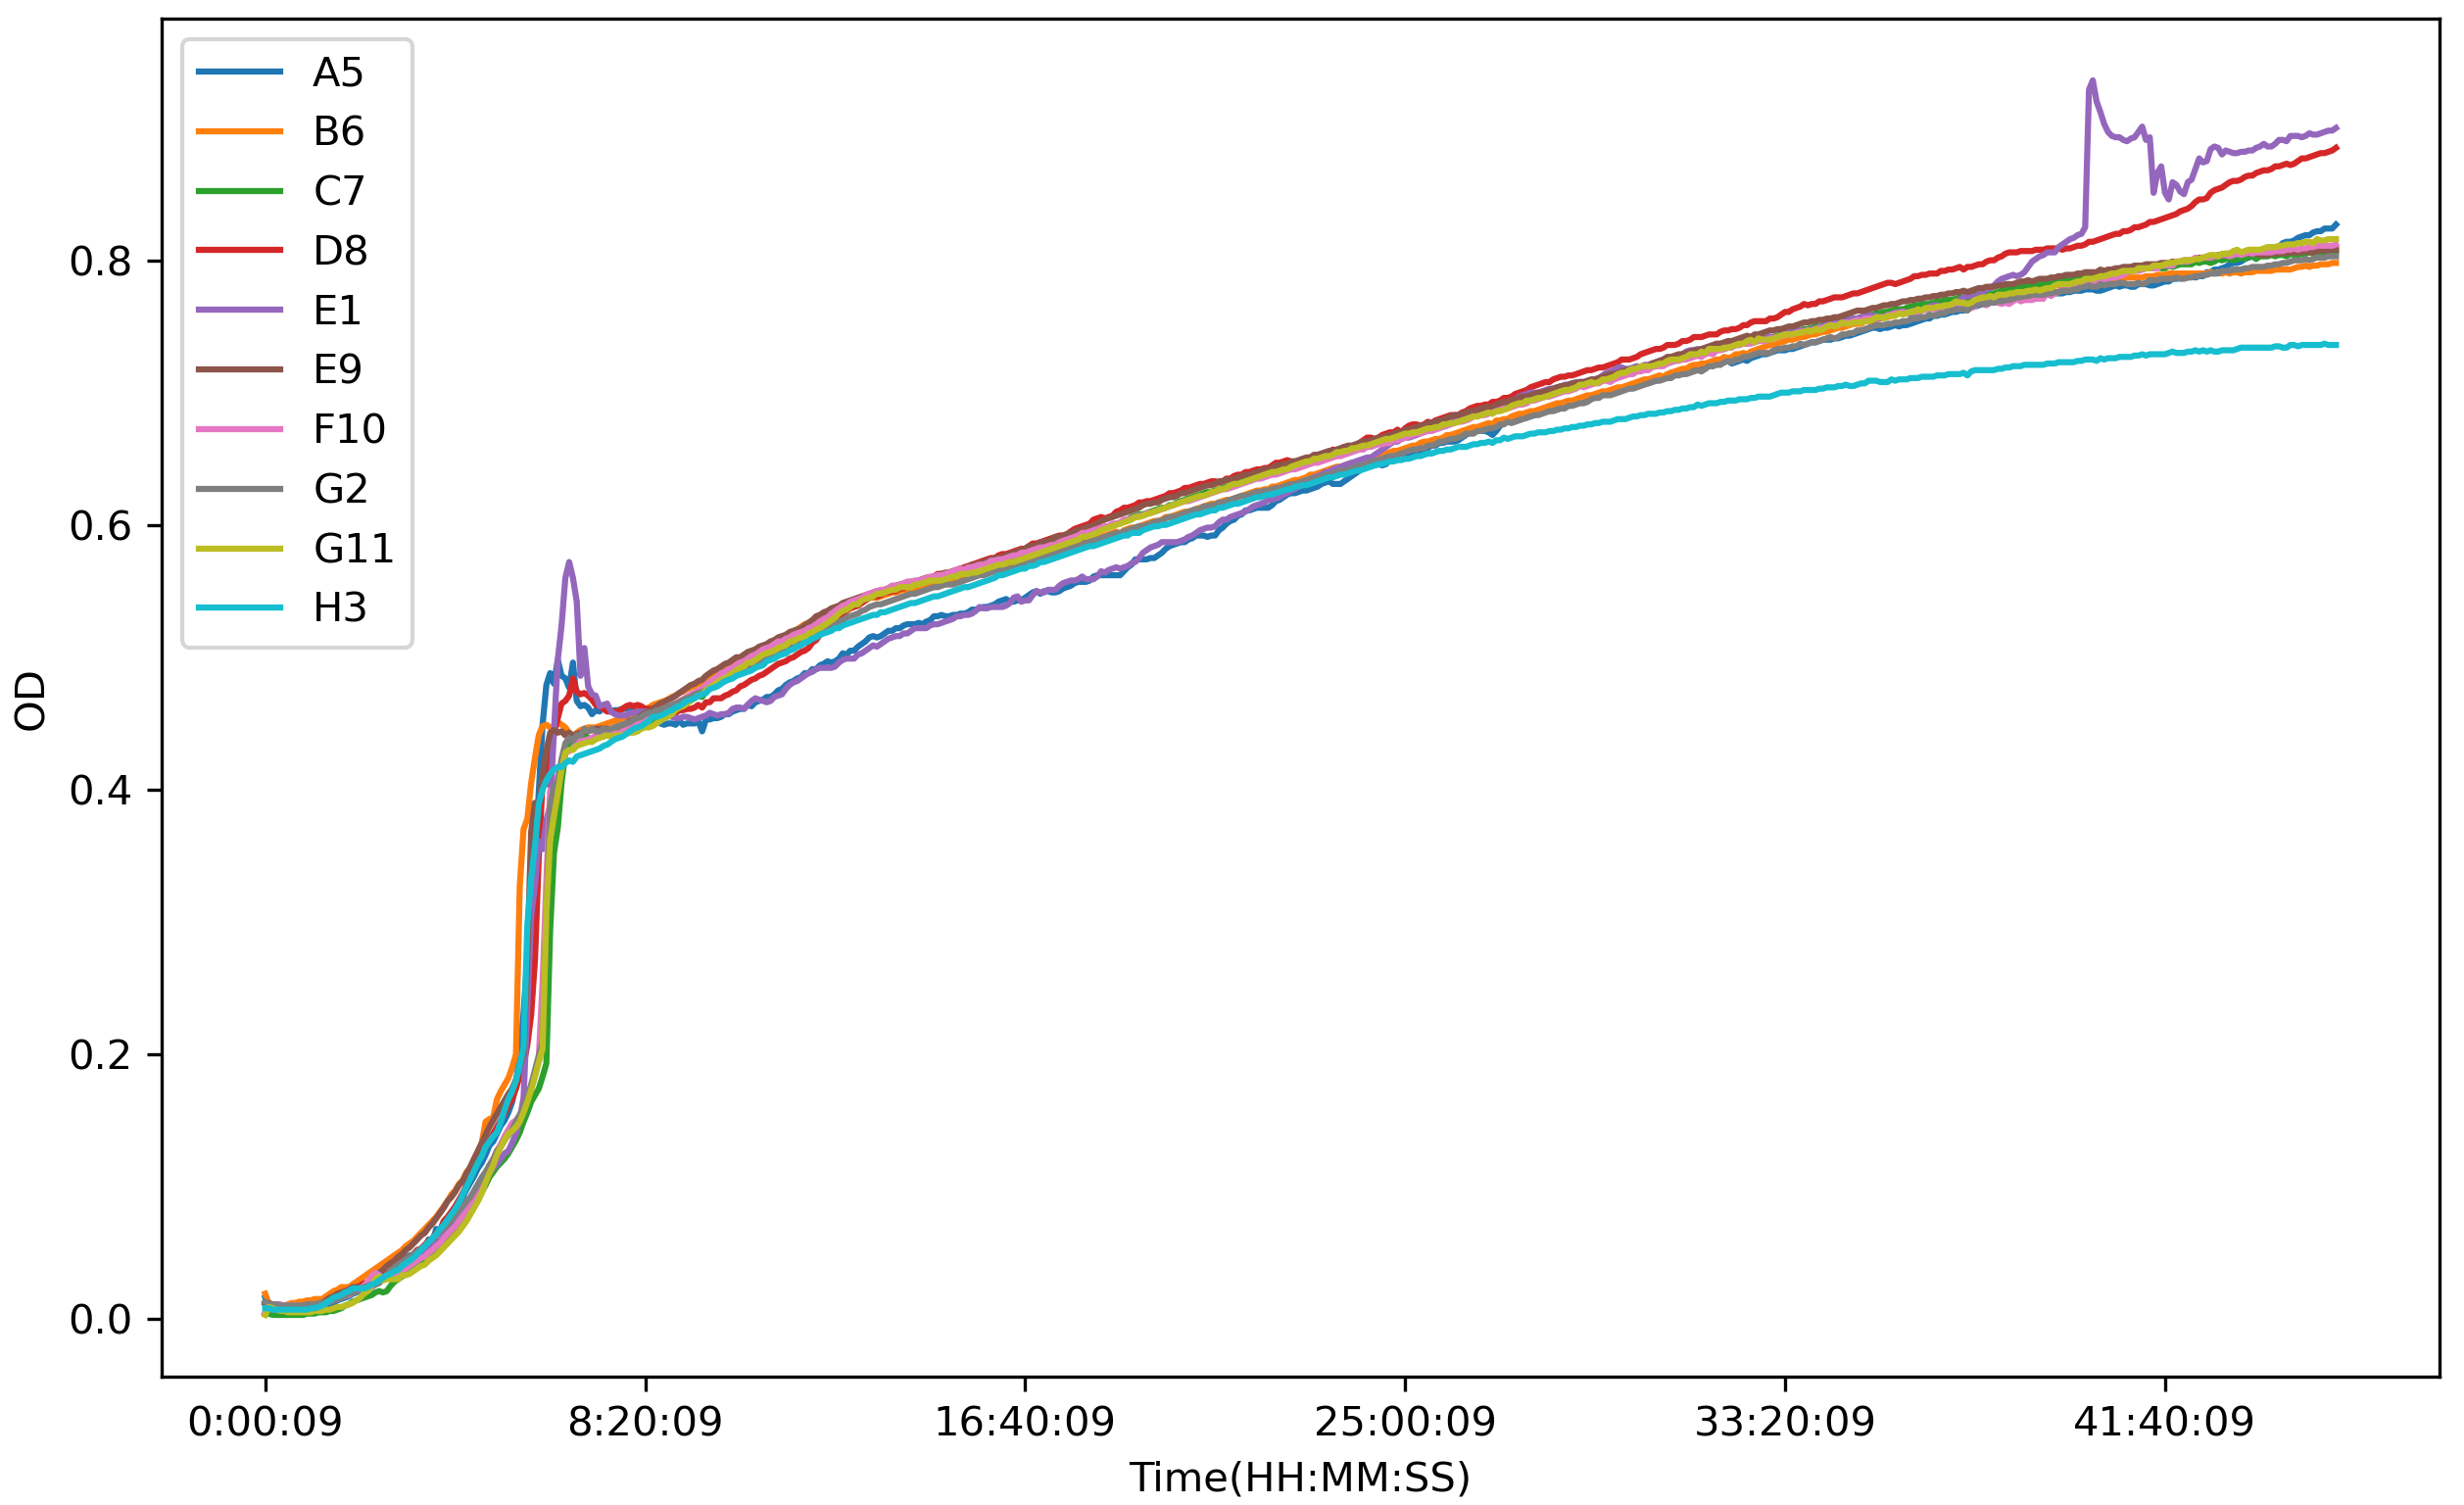
\includegraphics[scale = 0.7]{plots/gc.png}
    \caption{Growth curves for the wild type strain. Each curve represents a position in the 96 well plate}
    \label{fig:gc_wt}
\end{figure}

\subsection{Replication rates estimation from growth curves}

Determining growth rates from OD data is a process trickier than it looks; Ghenu and  some of the subtleties are discussed by Ghenu \cite{ghenu_challenges_nodate, krishnamurthi_new_2021}. 

Based on all the previous considerations, we fit a generalized logistic function (Eq \ref{eq:generalized_logistic}) to OD data for each plate's position. The fit was done with Scipy's optimize function, and further verified with lmfit package in python. 

\begin{equation}
    OD(t) = \frac{A}{\left(C + Q\exp{-Bx}\right)^\frac{1}{\nu}}
    \label{eq:generalized_logistic}
\end{equation}

It is possible to make a parallel with the parameters in \ref{eq:generalized_logistic} and the Logistic and Richardson models as proposed in \cite{ghenu_challenges_nodate}. Table \ref{tab:parameters_correspondence} shows the dependence between parameters of the different models 

\begin{table}
    \centering
    \begin{tabular}{|c|c|}
    \hline
    Logistic     & Richards\\
    \hline
    $\mu = B$     & $\mu = -\frac{B}{\nu}$\\
    $K = \frac{K}{K-1}Q$     & $K = A$\\
    $N_0 = \frac{1}{k-1}Q$     & $N_0 = \left(Q+1\right)^\frac{-1}{B}$\\
    $\nu = 1$     & $\nu = -B$\\
    $C = 1$ & $C = 1$\\
    \hline
    \end{tabular}
    \caption{Correspondence between the parameters for the Logistic and Richards models in \cite{ghenu_challenges_nodate} and the generalized logistic model (Eq \ref{eq:generalized_logistic}) used to fit OD curves}
    \label{tab:parameters_correspondence}
\end{table}

It is important to point out that this parallel holds only under the assumption that in the single scattering regime, OD values are proportional to the number of cells, $N$. In general, the relation between OD values and the number of cells is not well studied, it often requires calibration from the equipment used for each bacterial strain \cite{mira_estimating_2022}. Alternative experimental methods for estimating bacterial population from OD values have been suggested \cite{beal_robust_2020}; however, for the purposes of this project, we are not concerned with this problem directly. It is enough to restrict ourselves to the the single scattering regime, where we assume a linear relation between OD and N.

%Include table with fitted parameters for each strain type

\subsection{Solution to the model equations}
So far we haven't found an analytical solution to the equations; thus, we opted to analyze their stability and asymptotic behaviour. The first thing we looked at was the vector field in Fig \ref{fig:vector_field_2st} I found that there are only two equilibrium points, a unstable one at the origin $(F = M = 0)$ and a "degenerate attractor" along the line $F = K - M$. This "atractor" arises due to the carrying capacity term in the model. 
The trajectory way in which the system approaches this "attractor" depends on the initial conditions, as it can be see in Figure \ref{fig:2st_vector_fiel_with_trajectory} at the initial stages of the experiment, when the mutant population is zero, the systems approaches horizontally to the line; as the days pass and the starting mutant population increases, the system approaches the line more diagonally and eventually almost straight vertically. Furthermore, we observed that once the system reaches the line, it doesn't fluctuate and the only way for it to reset is by intervention through the dilutions.

\begin{figure}
    \centering
    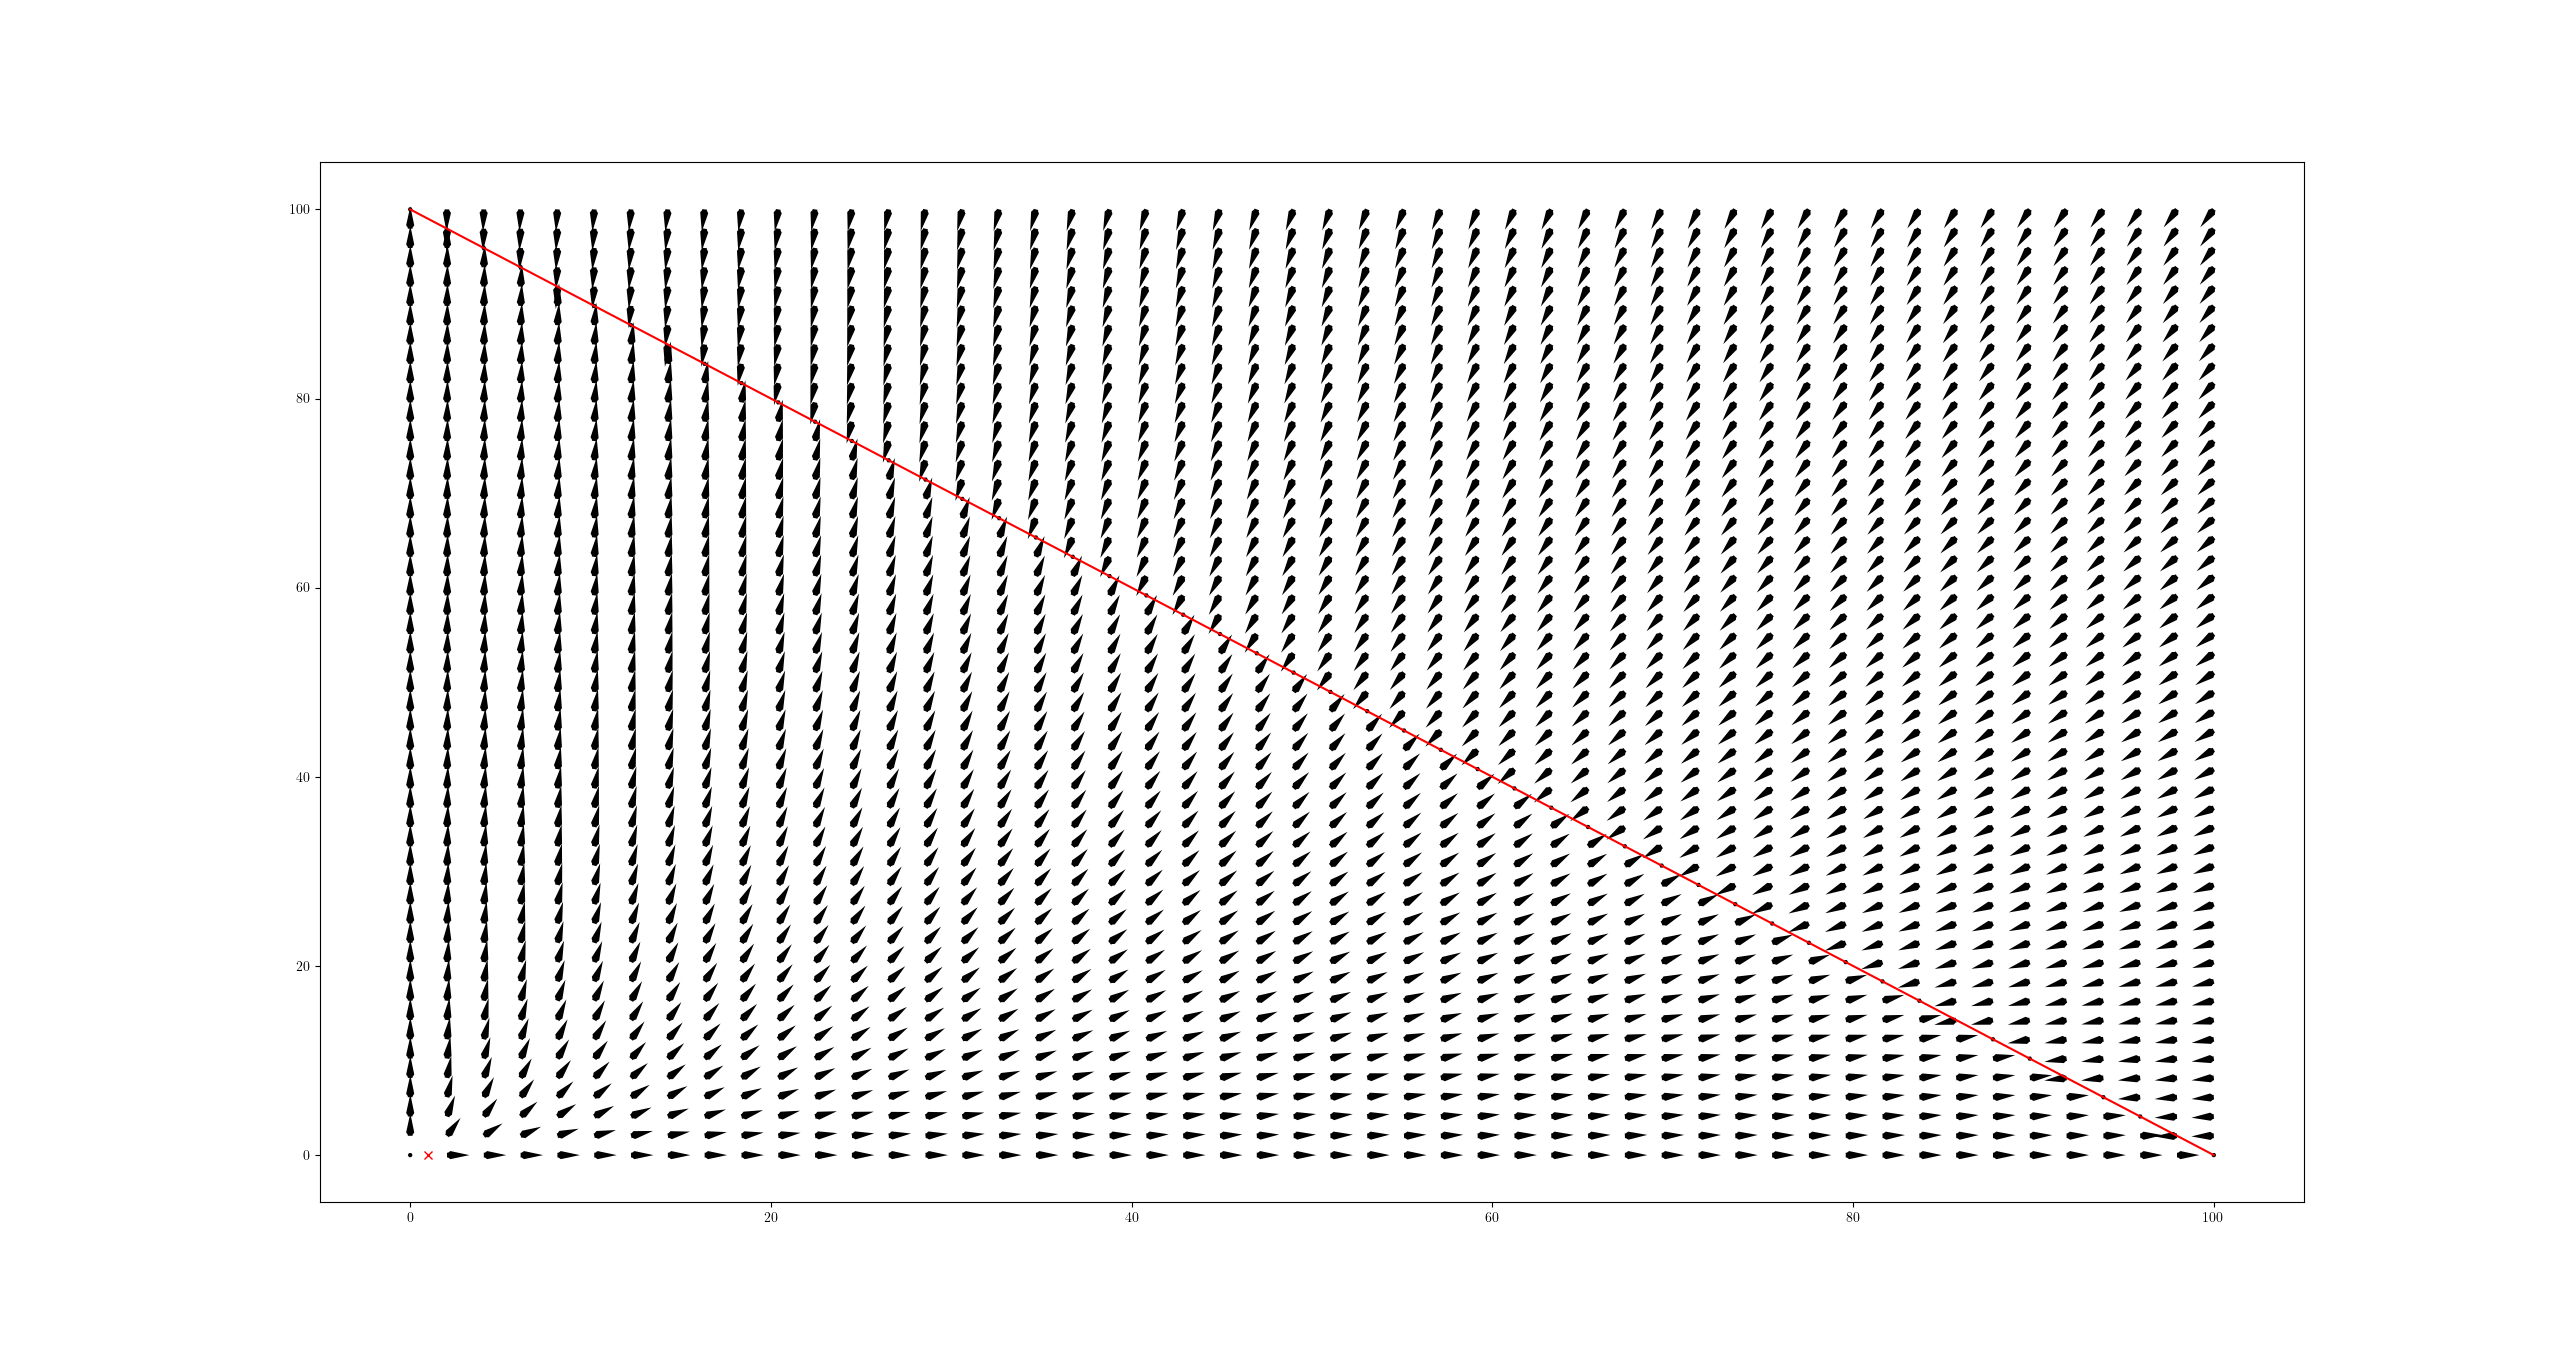
\includegraphics[width=1\linewidth]{plots/vector_field.png}
    \caption{Vector field plot for Eq \ref{eqs:adimensional_two_state_model}}
    \label{fig:vector_field_2st}
\end{figure}

Figure \ref{fig:2st_vector_fiel_with_trajectory} shows the trajectory in the phase space for a set of parameters with an appropriate order of magnitude inferred by comparison with the experimental data. The darker colors represent the first days of the experiment, here the population growth is mostly for the founder. Consecutive dilutions shift the initial point of the new trajectories, and cause a rapid increase for the mutant population, which after around 15 days takes over the system. Nonetheless, the founder strain does not extinguish and there is a remnant in agreement with the experiment.

\begin{figure}[H]
    \centering
    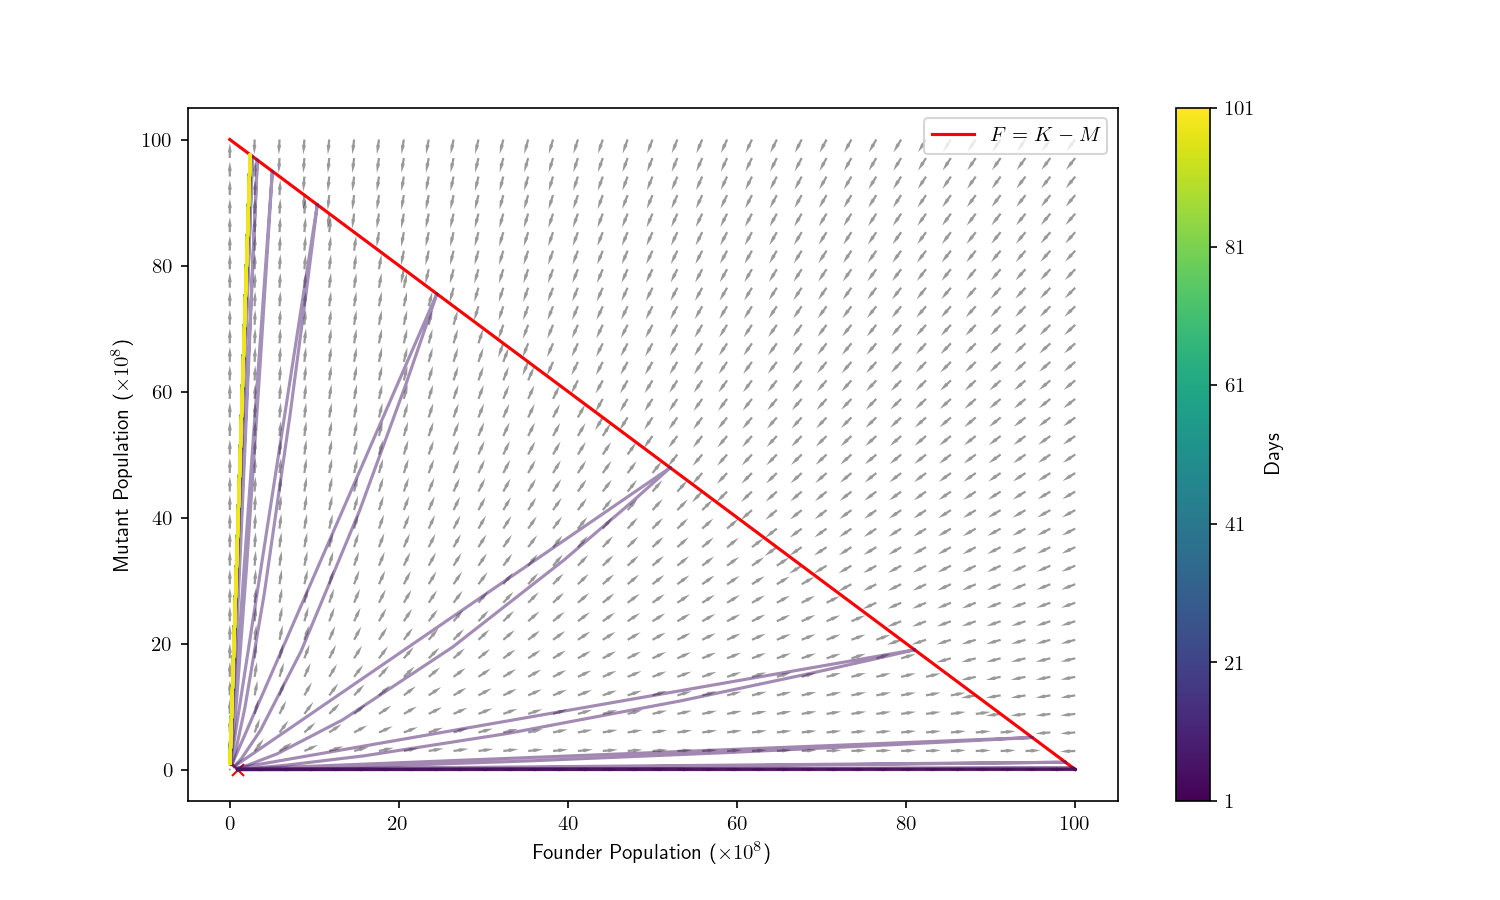
\includegraphics[width=1\linewidth]{plots/vector field with trajectory.png}
    \caption{Phase space trajectory for the two state system. The colors indicate the day of the experiment, darker colors indicate the earlier days and brighter the latter ones. The system rapidly goes from the initial state with mostly founders to the final state where there is coexistence between mutant and founder, with a higher abundance of the former.}
    \label{fig:2st_vector_fiel_with_trajectory}
\end{figure}

Now, in Fig \ref{fig:population_frac_2st} I look at the solution for the two state system\footnote{Even though we illustrate the behavior with replicate 1, the discussion is still valid for the other replicates as their values almost the same}. The sharp drops in the proportions of founder and mutant are captured, as well as the remnant population in the equilibrium state
\begin{figure}[H]
    \centering
    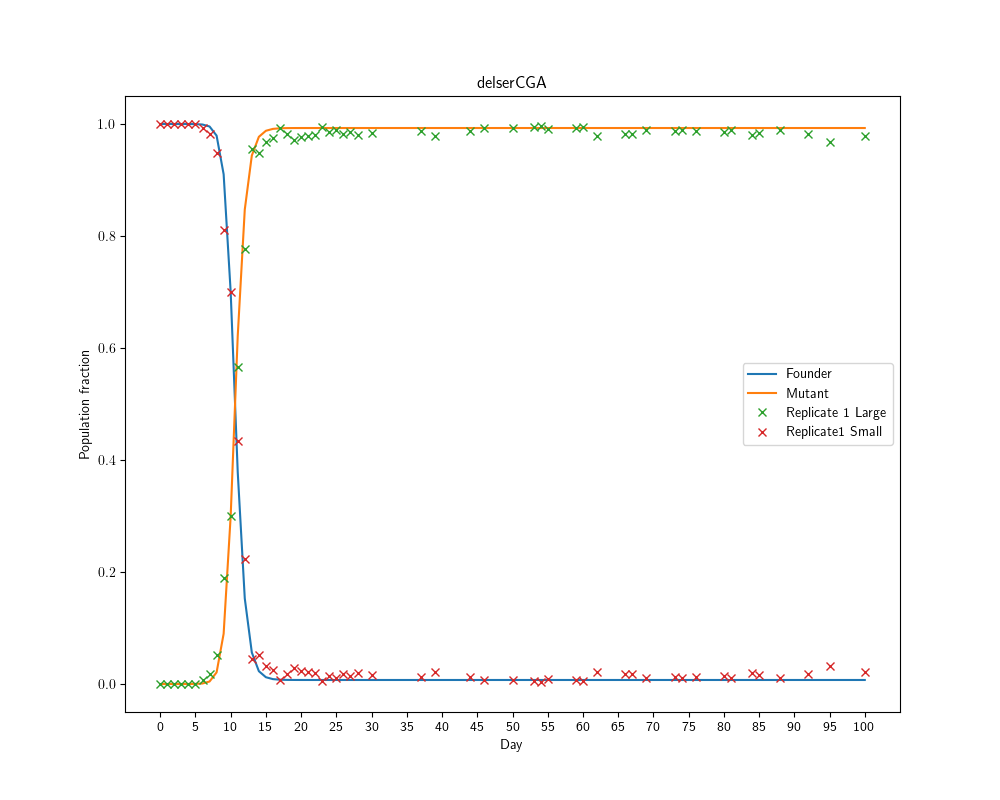
\includegraphics[width=1\linewidth]{guessed_params_2st_evolution_plot.png}
    \caption{Population fractions for the two state system. The parameters used were $K = 10^2$, $\alpha = 1.34187, \Tilde{mu}_{FM} = 0.0039\times 10^{-6}, \Tilde{mu}_{MF} = 1.26611\times 10^{-3}$. The solid lines are the theoretical predictions for the populations through the duration of the experiment. The x indicate the measured values of the populations proportions for small and large bacteria in Replicate 1. Large colonies are interpreted as encompassing all types of mutations, while small bacteria are understood as founder colonies.}
    \label{fig:population_frac_2st}
\end{figure}
The evolution experiment is carried out with the following conditions: 
\begin{itemize}
    \item The carrying capacity is set to $K = 10^{10} \text{cells}$
    \item The estimated initial cell density is $N_0= 10^9 \ \text{cells/mL}$ in 100 $\mu \text{L}$ of solution
    \item After each day 1\% of the solution is used to start the next culture
    \item The founder strain is the named \textit{delserCGA} and the reference duplication mutant is \textit{M2lop}
\end{itemize}

To solve Eq \ref{eqs:adimensional_two_state_model} we need a proxy for the values of the transition rates $(\Tilde{\mu}_{FM}, \Tilde{\mu}_{MF})$ and the mutant replication rates

\subsection{Parameter inference}

To gain some understanding on the behaviour of the solutions to Eq. \ref{eqs:adimensional_two_state_model} with respect to the parameters, I initially solved the two state system for different values of $(\Tilde{\mu}_{FM}, \Tilde{\mu}_{MF})$, the value of $\alpha$ was initially fixed as the growth curve data allowed the determination of the growth rates. This naive search provided some useful observations.
I found that varying $\Tilde{\mu}_{FM}$ shifts the day at which the final populations of mutant and founder are the same, without noticeably changing the ratio of their populations at the end of the experiment, meaning that this transition rate determines how fast the founder population will disappear. Qualitatively, this makes sense for me, considering that at the beginning of the experiment, there are no mutants, therefore the transition rate from $F$ to $M$ is an important contributor to the quickly appearance of a mutant population

On the other hand, varying $\Tilde{\mu}_{MF}$ seems to strongly determine the final fraction of population at the end of the experiment. Figure \ref{fig:effect_of_varying_mu_mf} illustrates this behaviour, for a small $\Tilde{\mu}_{MF}$ the ratio of founder in the final state is considerably higher than the ratio of mutants. As $\Tilde{\mu}_{MF}$ increases, the final founder ratio increases as well. This might indicate that this parameter is a key determinant for the fate of each strain, and in consequence of the proposed set of hypotheses. 

\begin{figure}
    \centering
    \begin{subfigure}[b]{0.4\textwidth}
    \centering
    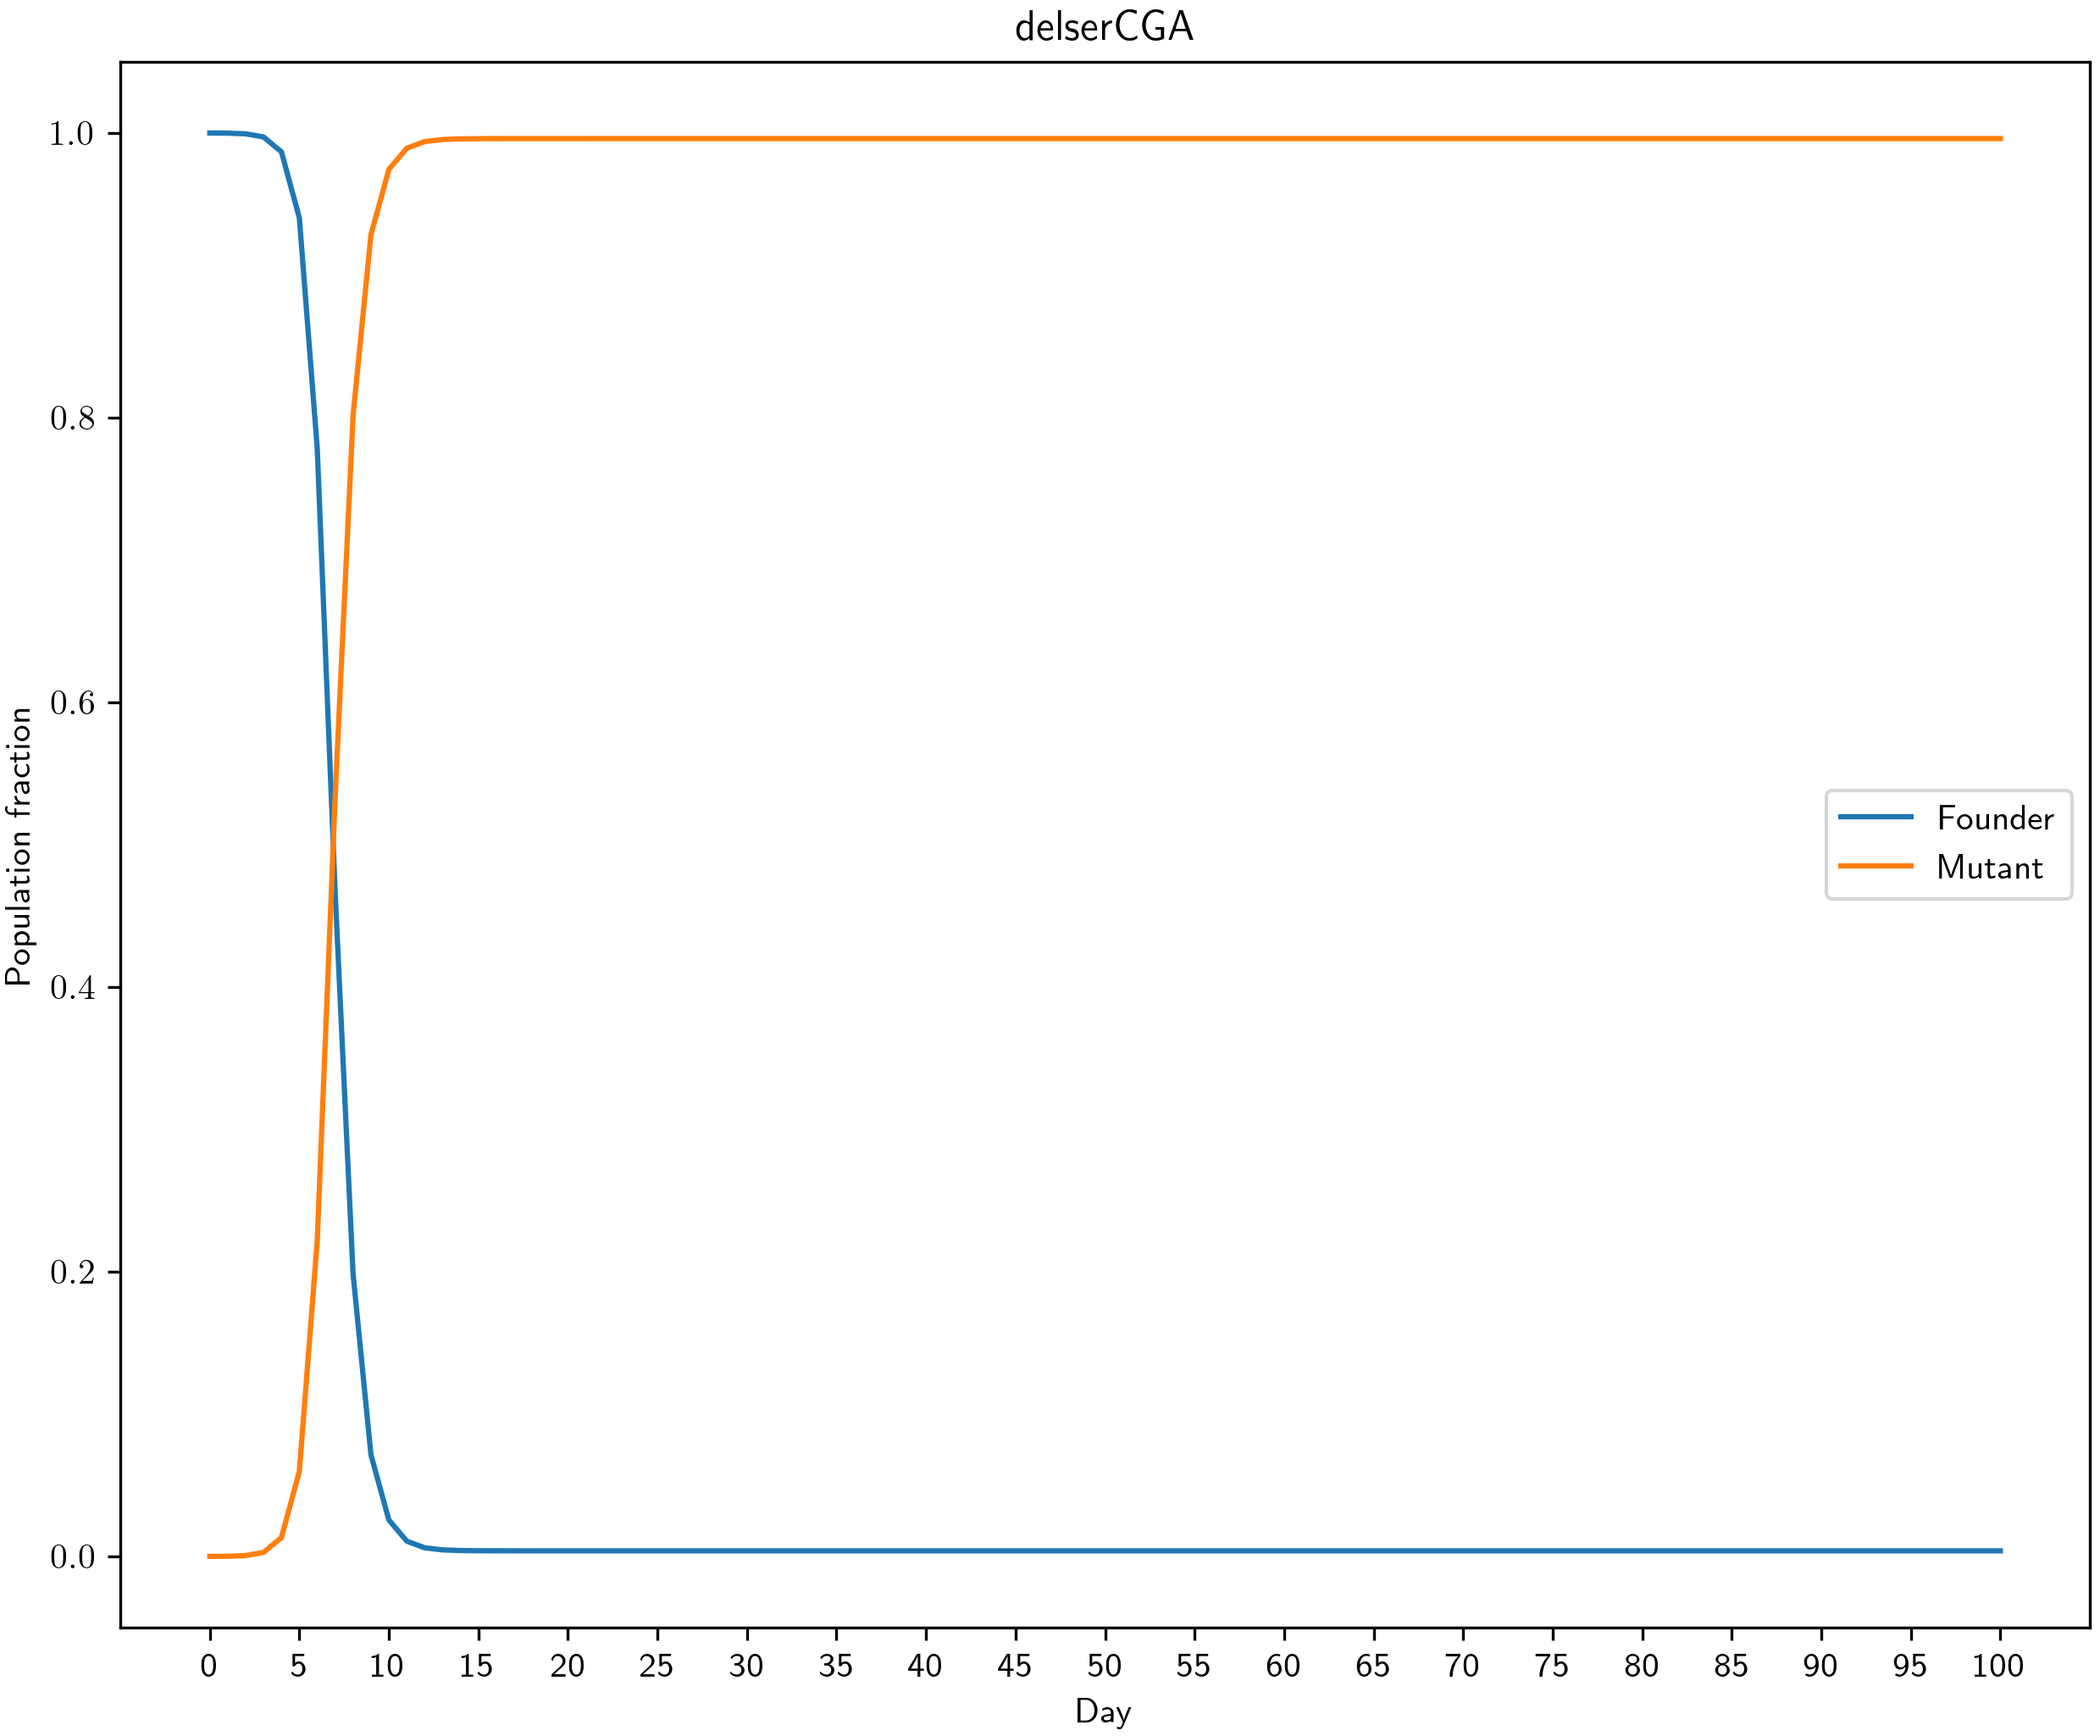
\includegraphics[scale=0.4]{plots/two_state_small_mu_mf.png}
    \end{subfigure}
    \hfill
    \begin{subfigure}[b]{0.4\textwidth}
    \centering
    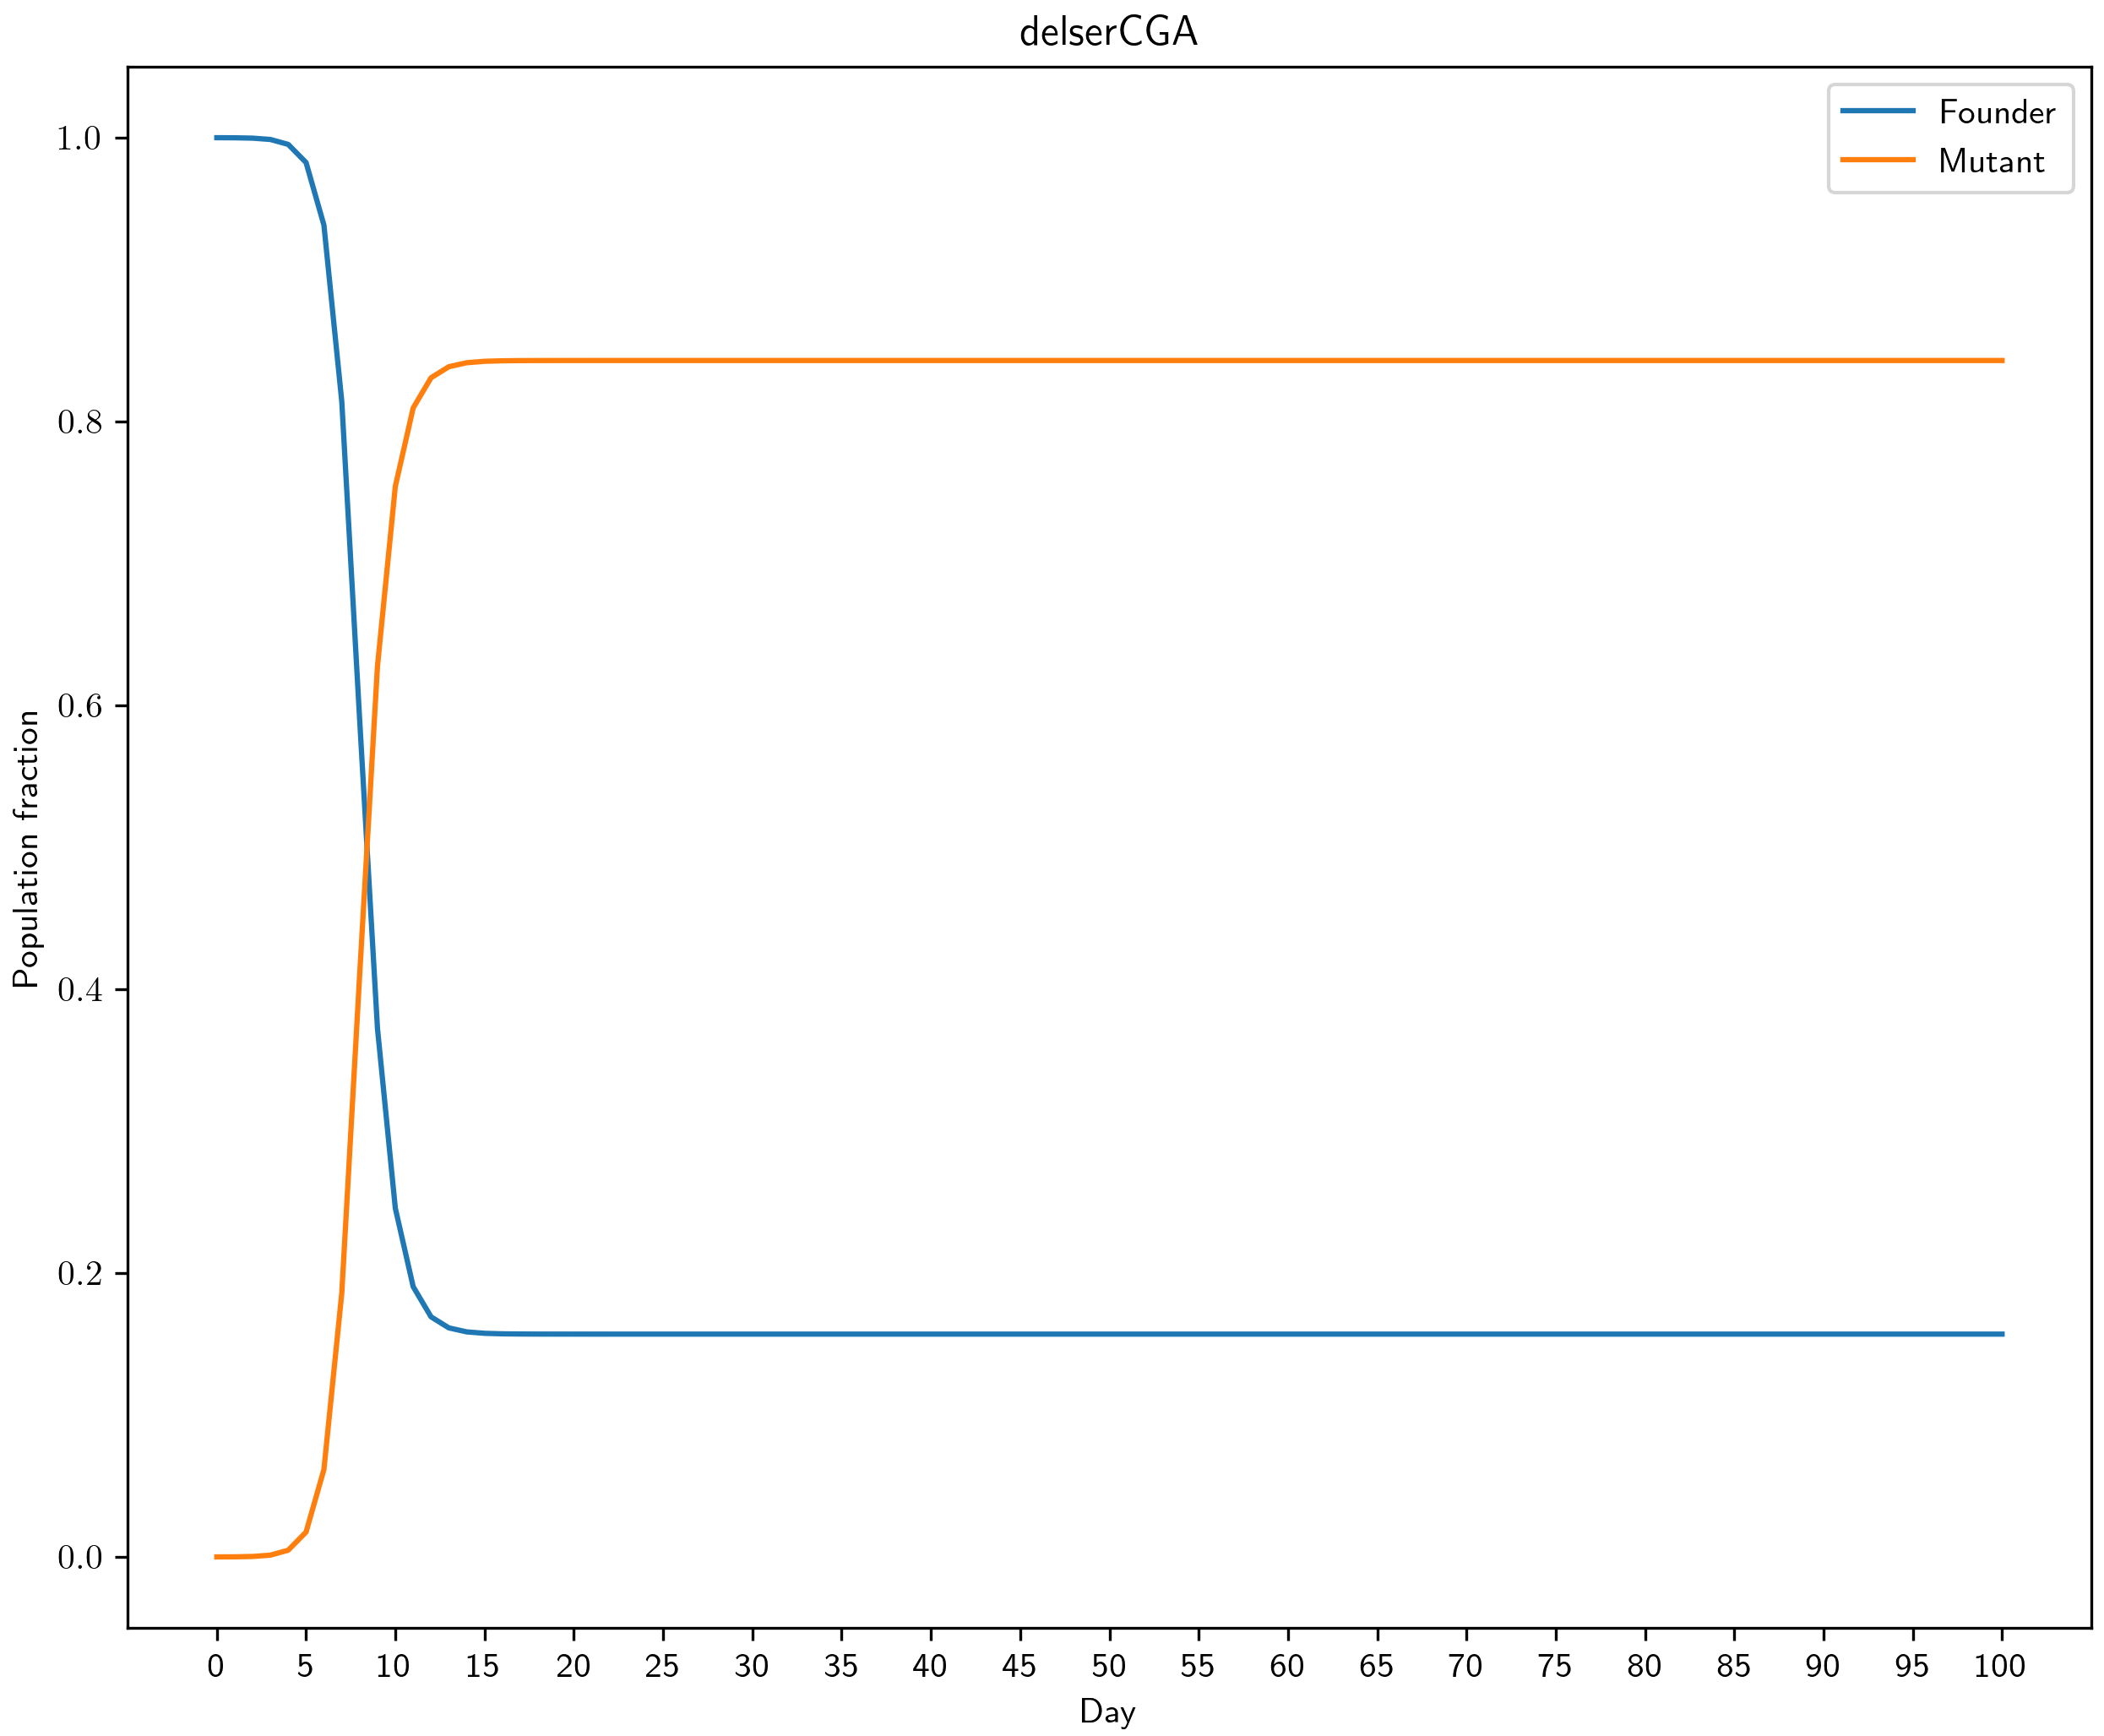
\includegraphics[scale=0.4]{plots/two_state_big_mu_mf.png}
    \end{subfigure}
    \caption{Effect of varying $\Tilde{\mu}_{MF}$ on the population fraction behavior in the evolution experiment. Both panels have fixed values for $\Tilde{\mu}_{FM}, \alpha$, $\Tilde{\mu}_{MF} = 0.001 * \ln{2}$ and bottom panel $\Tilde{\mu}_{MF} = 0.4 * \ln{2}$ }
    \label{fig:effect_of_varying_mu_mf}
\end{figure}

An important observation here is the difference in the order of magnitude for the transition rates,   $\Tilde{\mu}_{MF}$ has a stronger influence around $10^{-4}$, whereas $\Tilde{\mu}_{MF}$ does it around $10^{-9}$. Nonetheless, this behaviour is similar to the one described in \cite{reams_duplication_2010}

Now, when $\alpha$ is allowed to vary it exhibits a rather interesting behavior. In the limit where $\alpha \rightarrow 1$ there is no notorious shift in the population from founder and mutants; they remain close to their initial values, at least in a time frame suitable for an experiment. This behavior completely changes as $\alpha$ increases. As soon as $\alpha  \rightarrow 2$ the mutant population quickly takes over the system and remains like that for the rest of the experiment.

\subsubsection{Bayesian Inference for the two state model}
My initial approach to simplify the number of parameters to determine was to assume that the replication rate of the mutant was known, for this I used the value of the reported rate for \textit{M2lop} $(r_M = 0.05448 \text{ replication/min})$. By playing with the parameters I had some intuition about a range where the solution fit the experimental results (\ref{fig:population_frac_2st}). I chose to use Affine Invariant MCMC to determine the transition rates. With an uniform prior between 0 and 1 , the posterior distribution fails to reproduce similar experimental measurements.

Given that the initial flavor of MCMC was not successful at fitting the parameters to the experimental data, we switch to an Approximate Bayesian Calculation (ABC). This new approach yield satisfactory results shown in Figure \ref{fig:abc_2st_posterior}. This parameter distribution supports the values encountered previously for $\alpha$, and the difference between the orders of magnitude of mutation and loss rates is close to the behavior described in \cite{reams_duplication_2010} 
\begin{figure}[H]
	\centering
    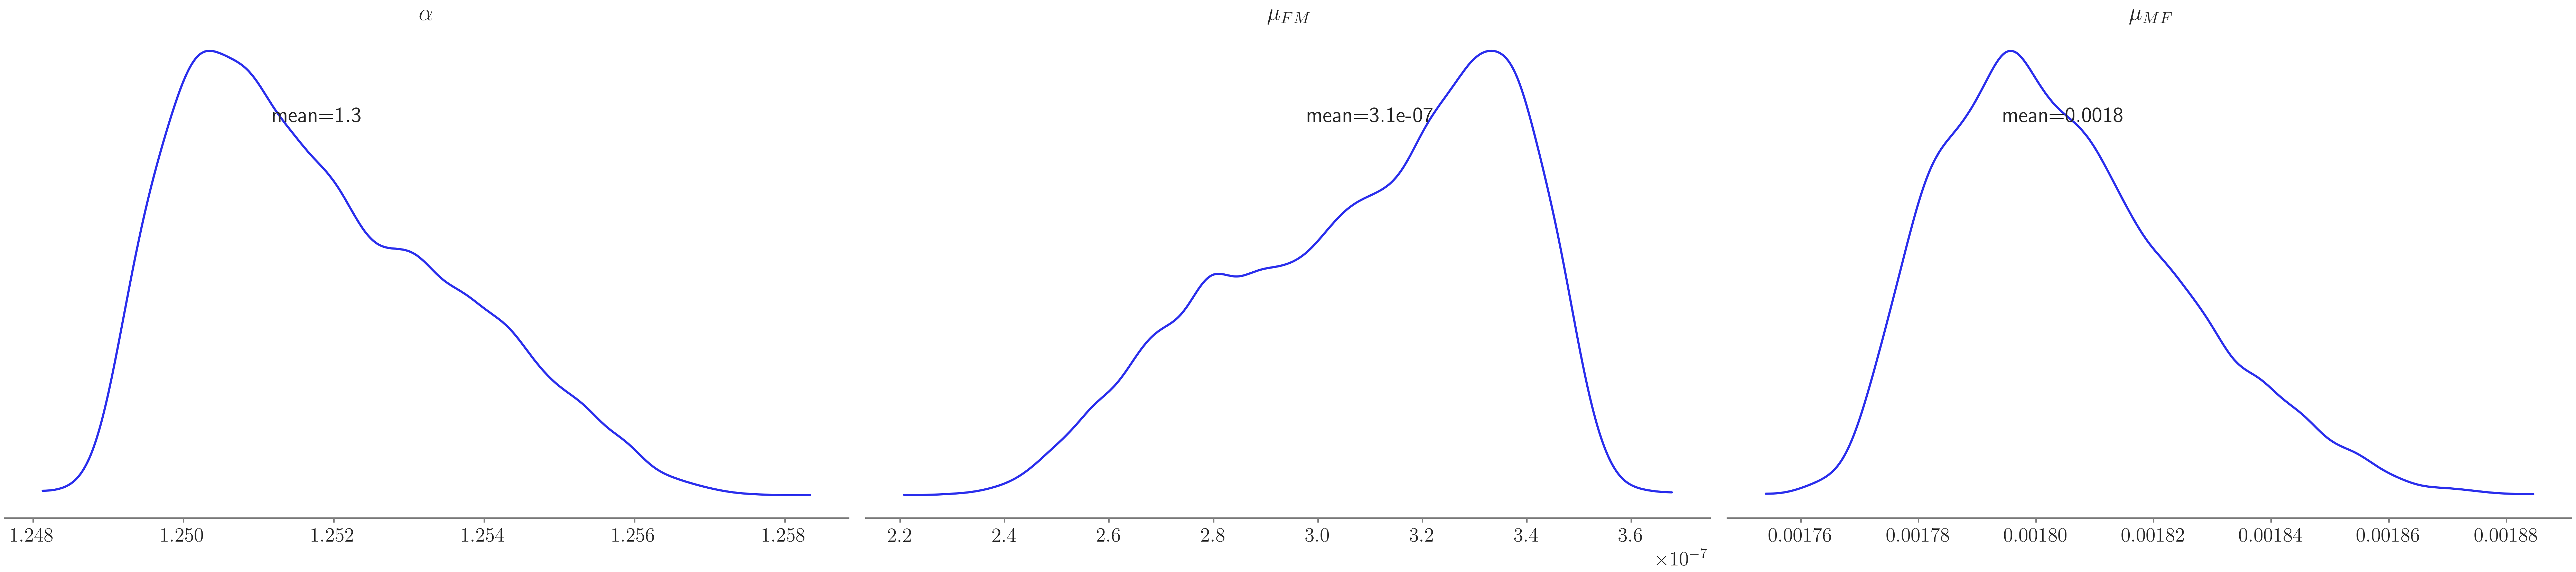
\includegraphics[scale=0.3]{plots/abc_2st_posterior.png}
    \caption{Posterior distribution for the parameters of the two state model inferred with ABC}
    \label{fig:abc_2st_posterior}
\end{figure}
Figure \ref{fig:2st_abc_fit} shows the experimental points along with the theoretical predictions (solid line) obtained by solving the model with the mean of the parameters distribution in Figure \ref{fig:abc_2st_posterior}. As we can see, the predictions reproduce the measured behavior of the populations, capturing the fast increase in mutants and the remnant founder population after 100 days.

\begin{figure}[H]
	\centering
    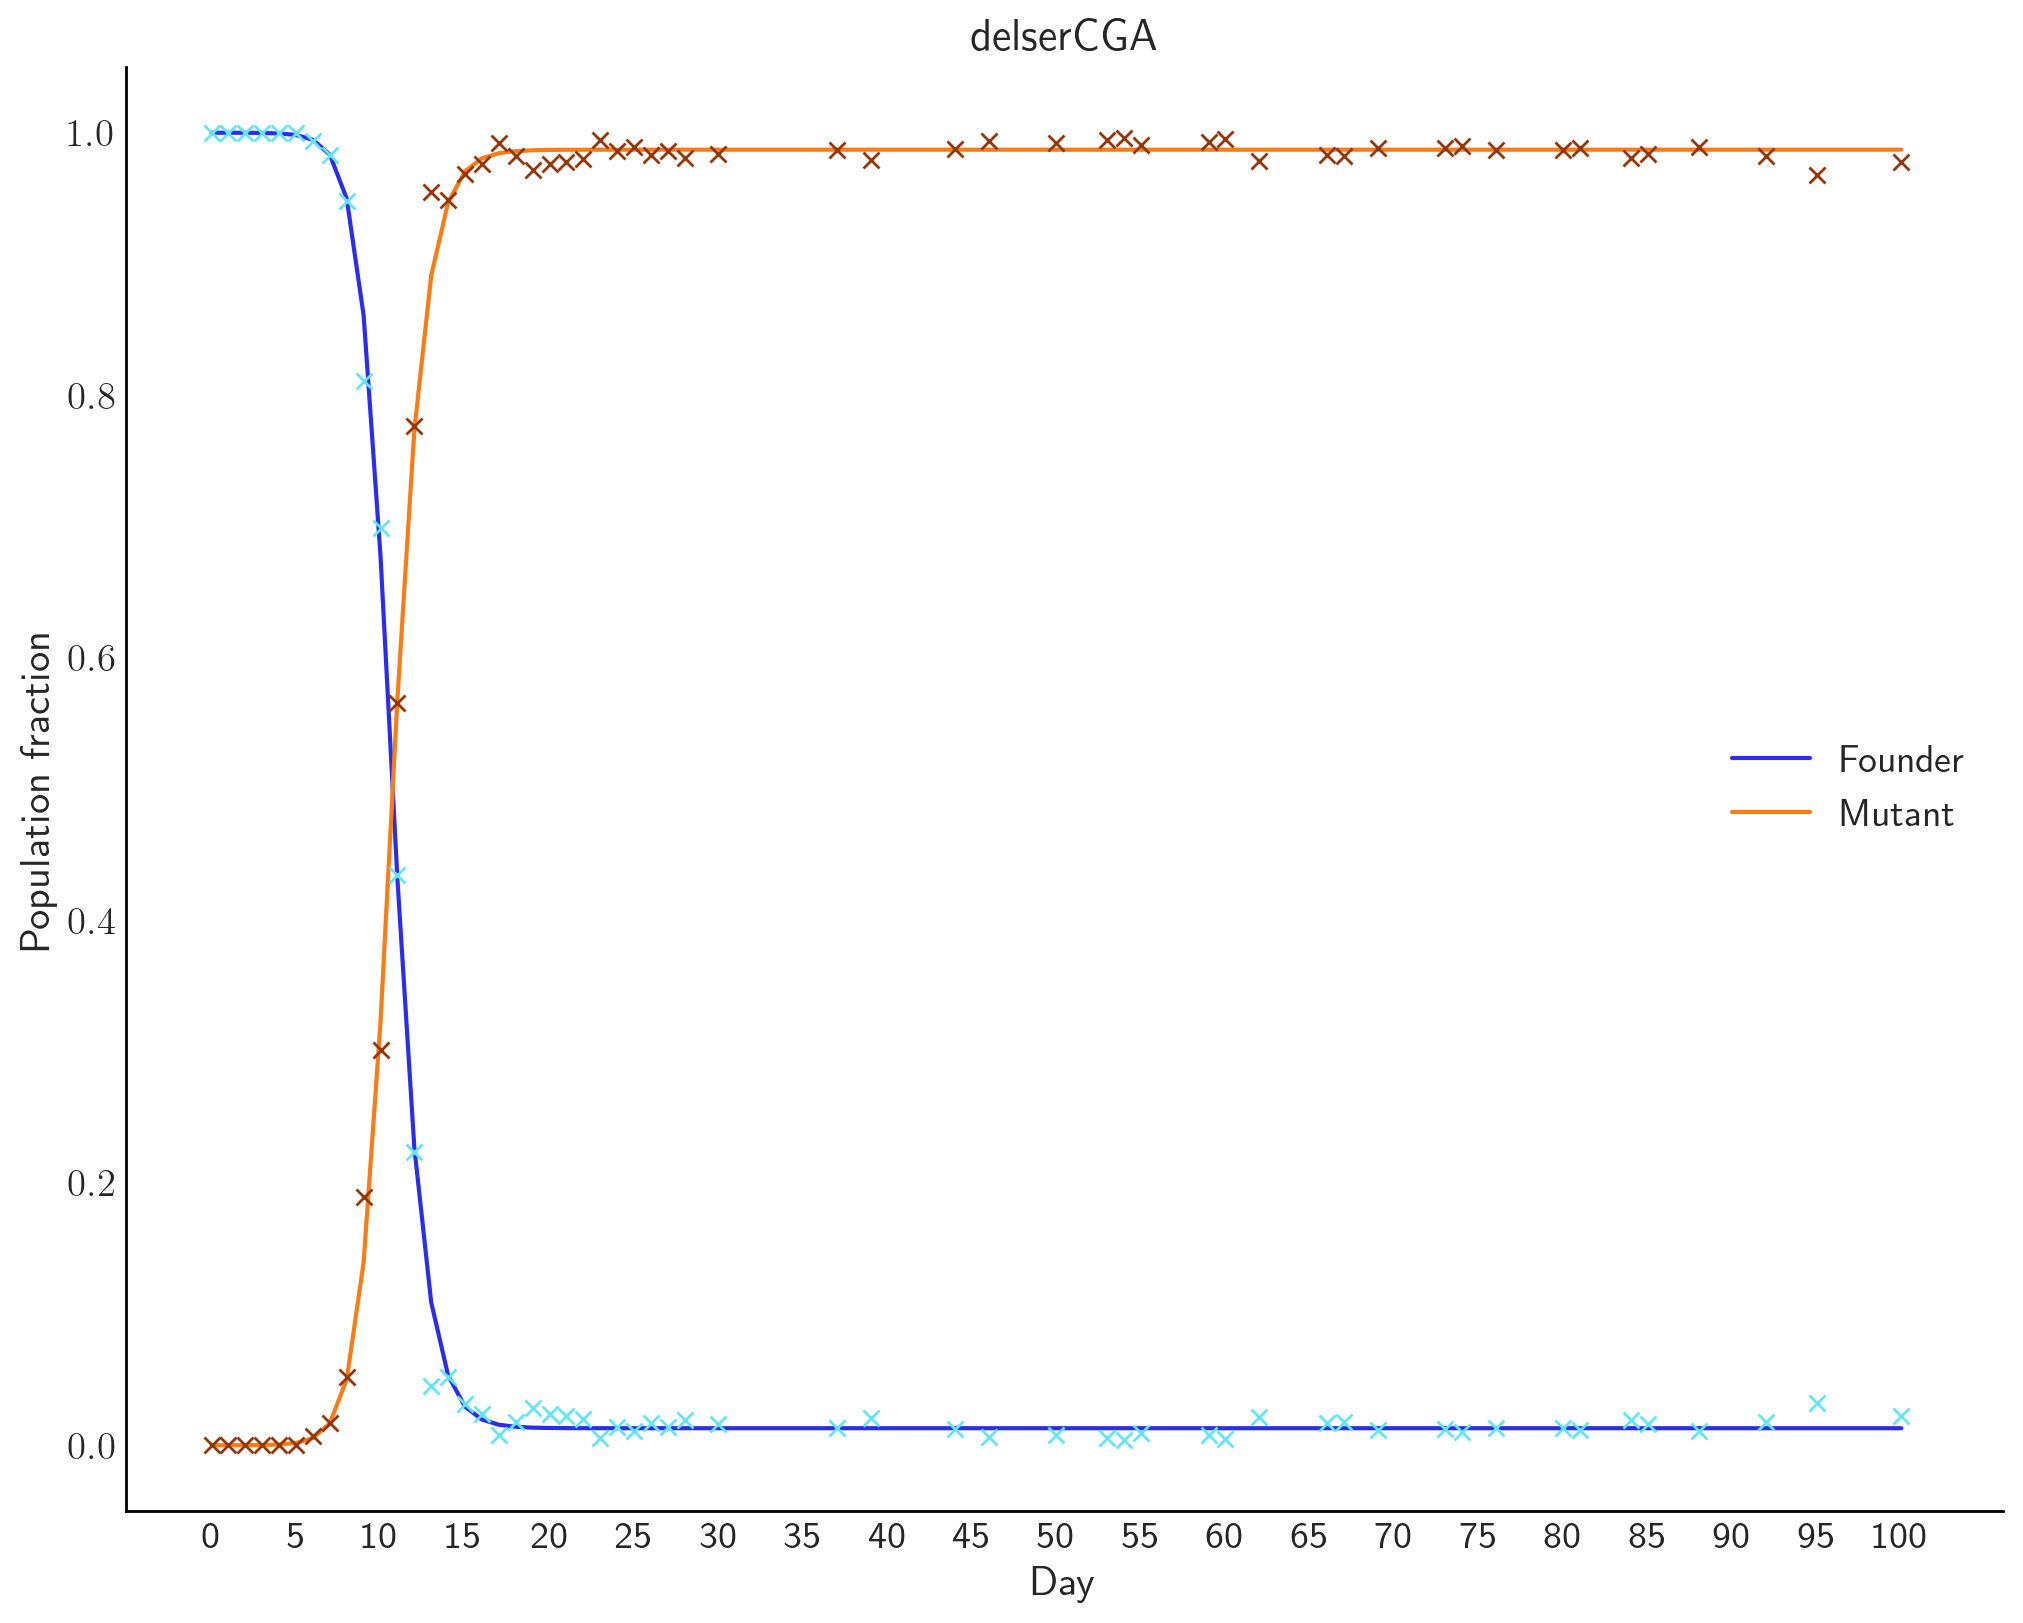
\includegraphics[scale=0.4]{plots/2st_abc_fit.png}
    \caption{The solid lines represent the theoretical evolution of the population fraction using the two state model. The x are the experimental measurements of the ratios of small and large colonies.}
    \label{fig:2st_abc_fit}
\end{figure}

\subsubsection{Bayesian Inference for the three state model}
Let's start by writing the adimensional expression of \ref{eqs:three_state_model}, where time has been scaled by a factor of $r_F$
\begin{subequations}\label{eqs:adimensional_three_state_model}
\begin{align}
\dv{F}{\tau} &= \left( \left(1 - \Tilde{\mu}_{FD} - \Tilde{\mu}_{FS}\right)F + \alpha \Tilde{\mu}_{DF} D + \beta \Tilde{\mu}_{SF} S \right)\left(1-\frac{F + D + S}{K}\right)\\
\dv{D}{\tau} &=\left(  \Tilde{\mu}_{FD}F + \alpha\left(1 -\Tilde{\mu}_{DF}\right)D \right) \left(1-\frac{F + D + S}{K}\right) \\
\dv{S}{\tau} &= \left( \Tilde{\mu}_{FS}F + \beta\left(1 - \Tilde{\mu}_{SF}\right)S \right) \left(1-\frac{F + D + S}{K}\right) 
\end{align}
\end{subequations}
with $\tau = r_F t$, $\alpha = \frac{r_D}{r_F}, \beta = \frac{r_S}{r_F}$, $\Tilde{\mu}_{FD} = \frac{\mu_{F\rightarrow D}}{\ln{2}}, \Tilde{\mu}_{FS} = \frac{\mu_{F\rightarrow S}}{\ln{2}}, \Tilde{\mu}_{DF} = \frac{\mu_{D\rightarrow F}}{\ln{2}}, \Tilde{\mu}_{SF} = \frac{\mu_{S\rightarrow F}}{\ln{2}}$.
This model involves more unknown parameters than Eq \ref{eqs:adimensional_two_state_model}, thus MCMC computation time will be significantly larger as it scales with the dimensionality of the parameter space. Running an Approximate Bayesian Computation algorithm is a more suitable option, given that it doesn't involve calculating a likelihood function and the implementation chosen is well optimized. From solving Eqs \ref{eqs:adimensional_three_state_model} for different combinations of parameters and previous work with the two state model, I already had prior knowledge of at least some orders of magnitude for the parameters. In this way I define the prior probability as
\begin{subequations}
    \begin{align*}
        \alpha, \beta &\sim \mathcal{U}_{[1,2]}\\
        \Tilde{\mu}_{FD} &\sim \mathcal{N}(0,10^{-5}), \quad \Tilde{\mu}_{FD}>0 \\
        \Tilde{\mu}_{FS} &\sim \mathcal{N}(0,10^{-5}), \quad \Tilde{\mu}_{FS}>0 \\
        \Tilde{\mu}_{DF} &\sim \mathcal{N}(0,10^{-5}), \quad \Tilde{\mu}_{DF}>0 \\
        \Tilde{\mu}_{SF} &\sim \mathcal{N}(0,10^{-5}), \quad \Tilde{\mu}_{SF}>0 
    \end{align*}
\end{subequations}

The ABC calculations yield the following posterior distribution for the parameters. converge to the following parameter distribution, Fig \ref{fig:posterior_abc_3st}

\begin{figure}[H]
    \centering
    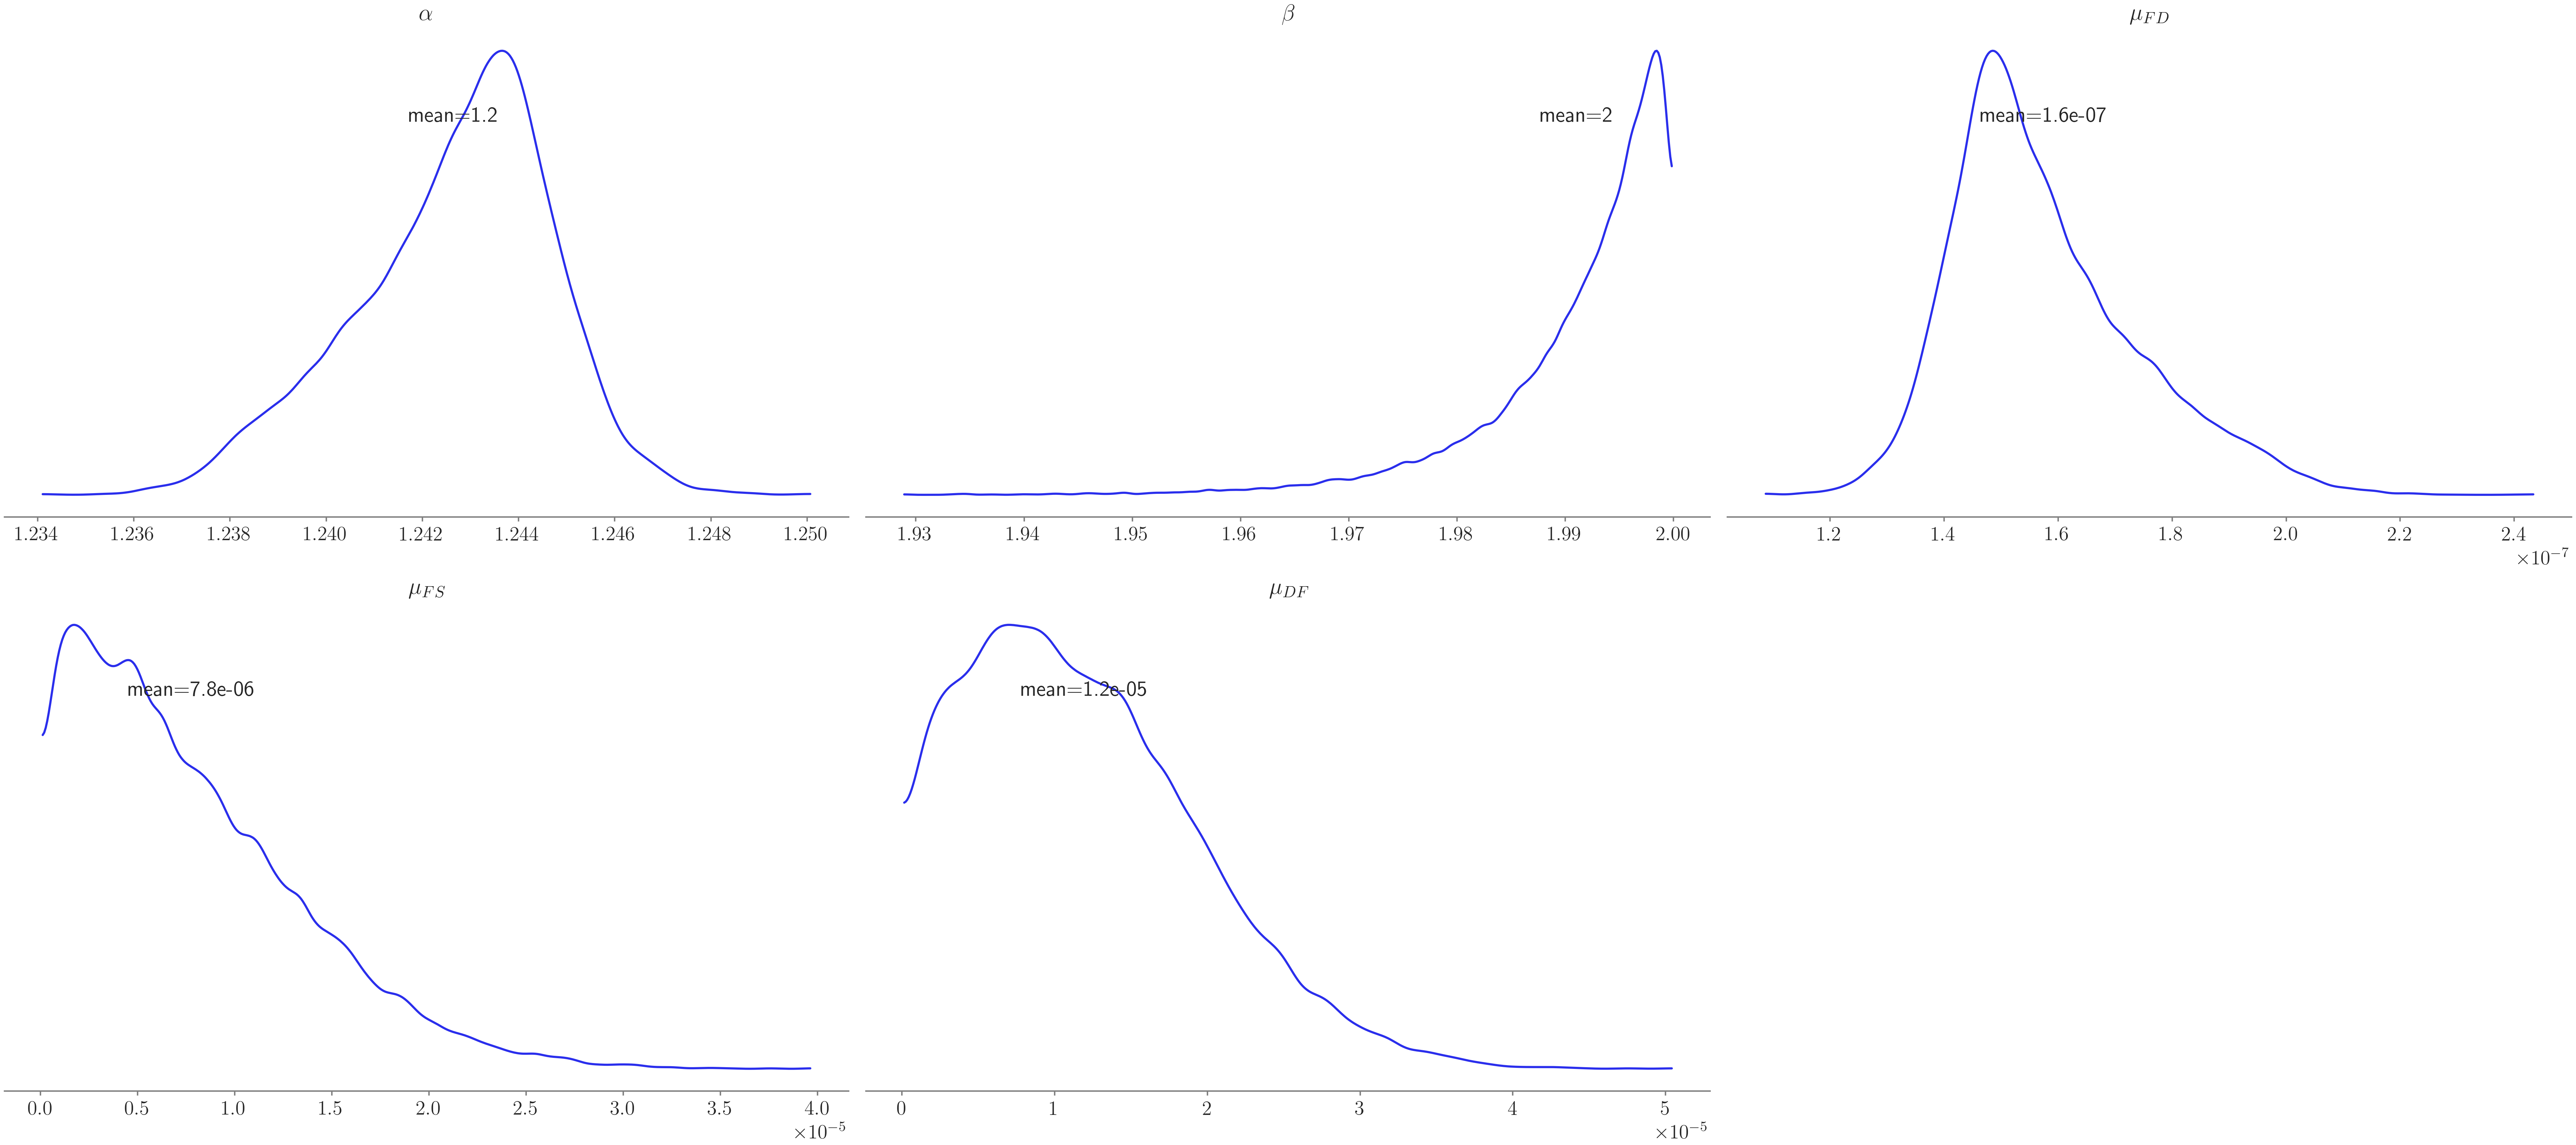
\includegraphics[width=1\linewidth]{abc_3st_posterior.png}
    \caption{Posterior distribution for parameters in Eq \ref{eqs:adimensional_three_state_model}}
    \label{fig:posterior_abc_3st}
\end{figure}

Even though we had a value for the replication rate of the \textit{M2lop} mutant, we set it to vary in the model. Table \ref{tab:abc_3st_params} summarizes the mean and std of each distribution.

\begin{table}[H]
    \centering
    \begin{tabular}{c|c|c}
    \hline
    & \textbf{mean} & \textbf{std} \\\hline
     $\alpha$ & 1.2427   & $2.0 \times 10^{-3}$ \\
     $\beta$  & $1.9911$ & $8.5 \times 10^{-3}$\\
     $\mu_{FD}$    & $1.576\times 10^{-7}$ & $1.634\times 10^{-8}$ \\
     $\mu_{FS}$    & $7.811\times 10^{-6}$ & $5.804\times 10^{-6}$ \\
     $\mu_{DF}$    & $1.199\times 10^{-5}$ & $7.598\times 10^{-6}$ \\\hline
    \end{tabular}
    \caption{Statistics summary of the parameter distribution for Eq \ref{eqs:adimensional_three_state_model} from ABC results}
    \label{tab:abc_3st_params}
\end{table}

I choose the mean of each parameter as a representative sample of the algorithm results, and use them solve the experiment. To compare with the experimental data, I sum the population fractions from Duplication and SNP strains, this should correspond to the fraction of observed large colonies. Visually inspecting the population fractions in Fig \ref{fig:abc_3st_experiment_comparison} we can see that the prediction with the inferred parameters is close to the experimental data. Furthermore, the parameters seem to reproduce the long-time behaviour of the experiment as there is the founder population is not completely extinguished, instead there is a small remnant of it.
\begin{figure}[H]
    \centering
    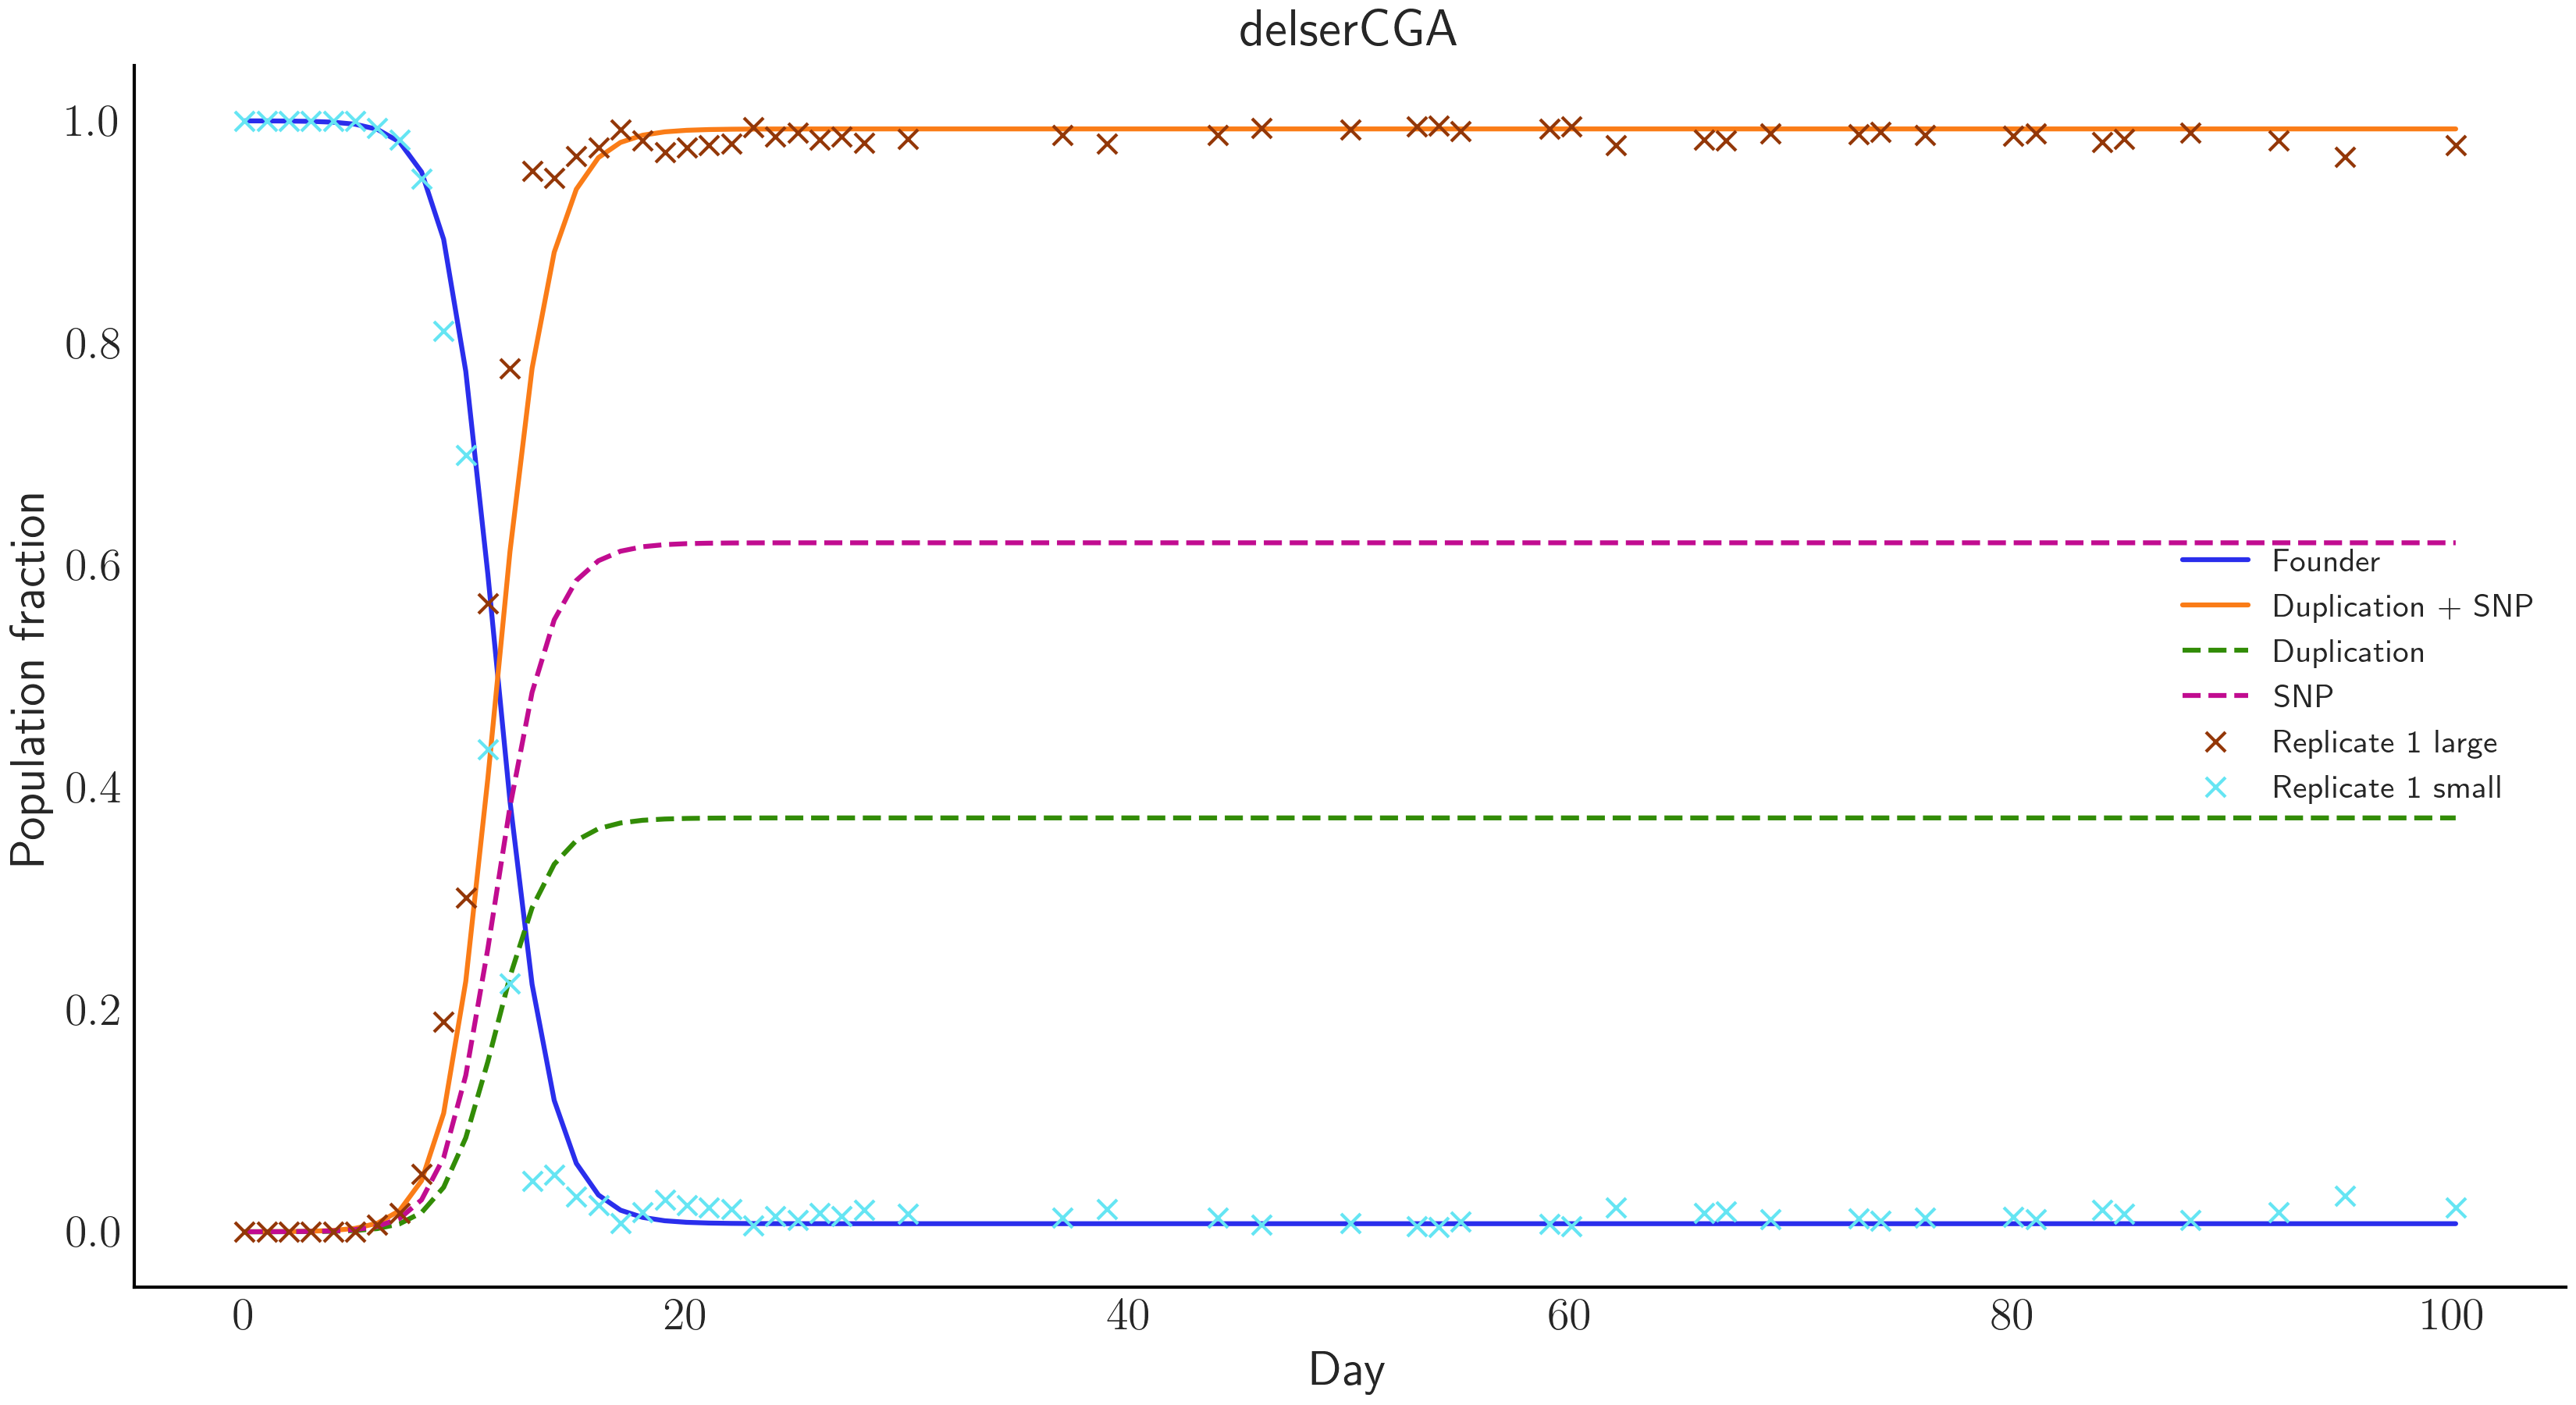
\includegraphics[width=1\linewidth]{plots/abc_3st_experiment_comparison.png}
    \caption{Sample of the experiment results using the mean of the parameters distribution}
    \label{fig:abc_3st_experiment_comparison}
\end{figure}

Furthermore, this plot shows that in the end, there is a stable equilibrium between SNP, Duplication and Founder strains with SNP being the dominant one. Moreover, this result does not completely support any of the hypotheses, perhaps signalling that it is necessary to review and update them.

Nonetheless, these are exciting results as now we seem to be able to estimate a reasonable value from the parameters. We can use this information to impose constraints in the parameter space when carrying out calculations for the time to reach the equilibrium.

\subsection{Parameter space exploration}

We explore the parameter space of our models to analyze the time to the steady state, and the fate of the different strains. We start by looking at the two state model; based on our previous work we know that the two parameters which determine the dynamics of the system are the ratio of the replication rates $(\alpha = r_M / r_F)$ and the mutation loss rate $\mu_{MF}$. Using the results of our inference task we restrict the search interval to $10^{-3} \leq \mu_{MF} \leq 2 \times 10^{-1}$ and $1 \leq \alpha \leq 2$

We say that the system has reached the steady state\footnote{The simulation ran for a maximum of 1000 days, in case that convergence was not achieved prior to that point, we show the max number of steps as the convergence time} when the variation of the population for three consecutive days is smaller than a set threshold of $\epsilon = 10^{-5}$

\begin{figure}[H]
	\centering
	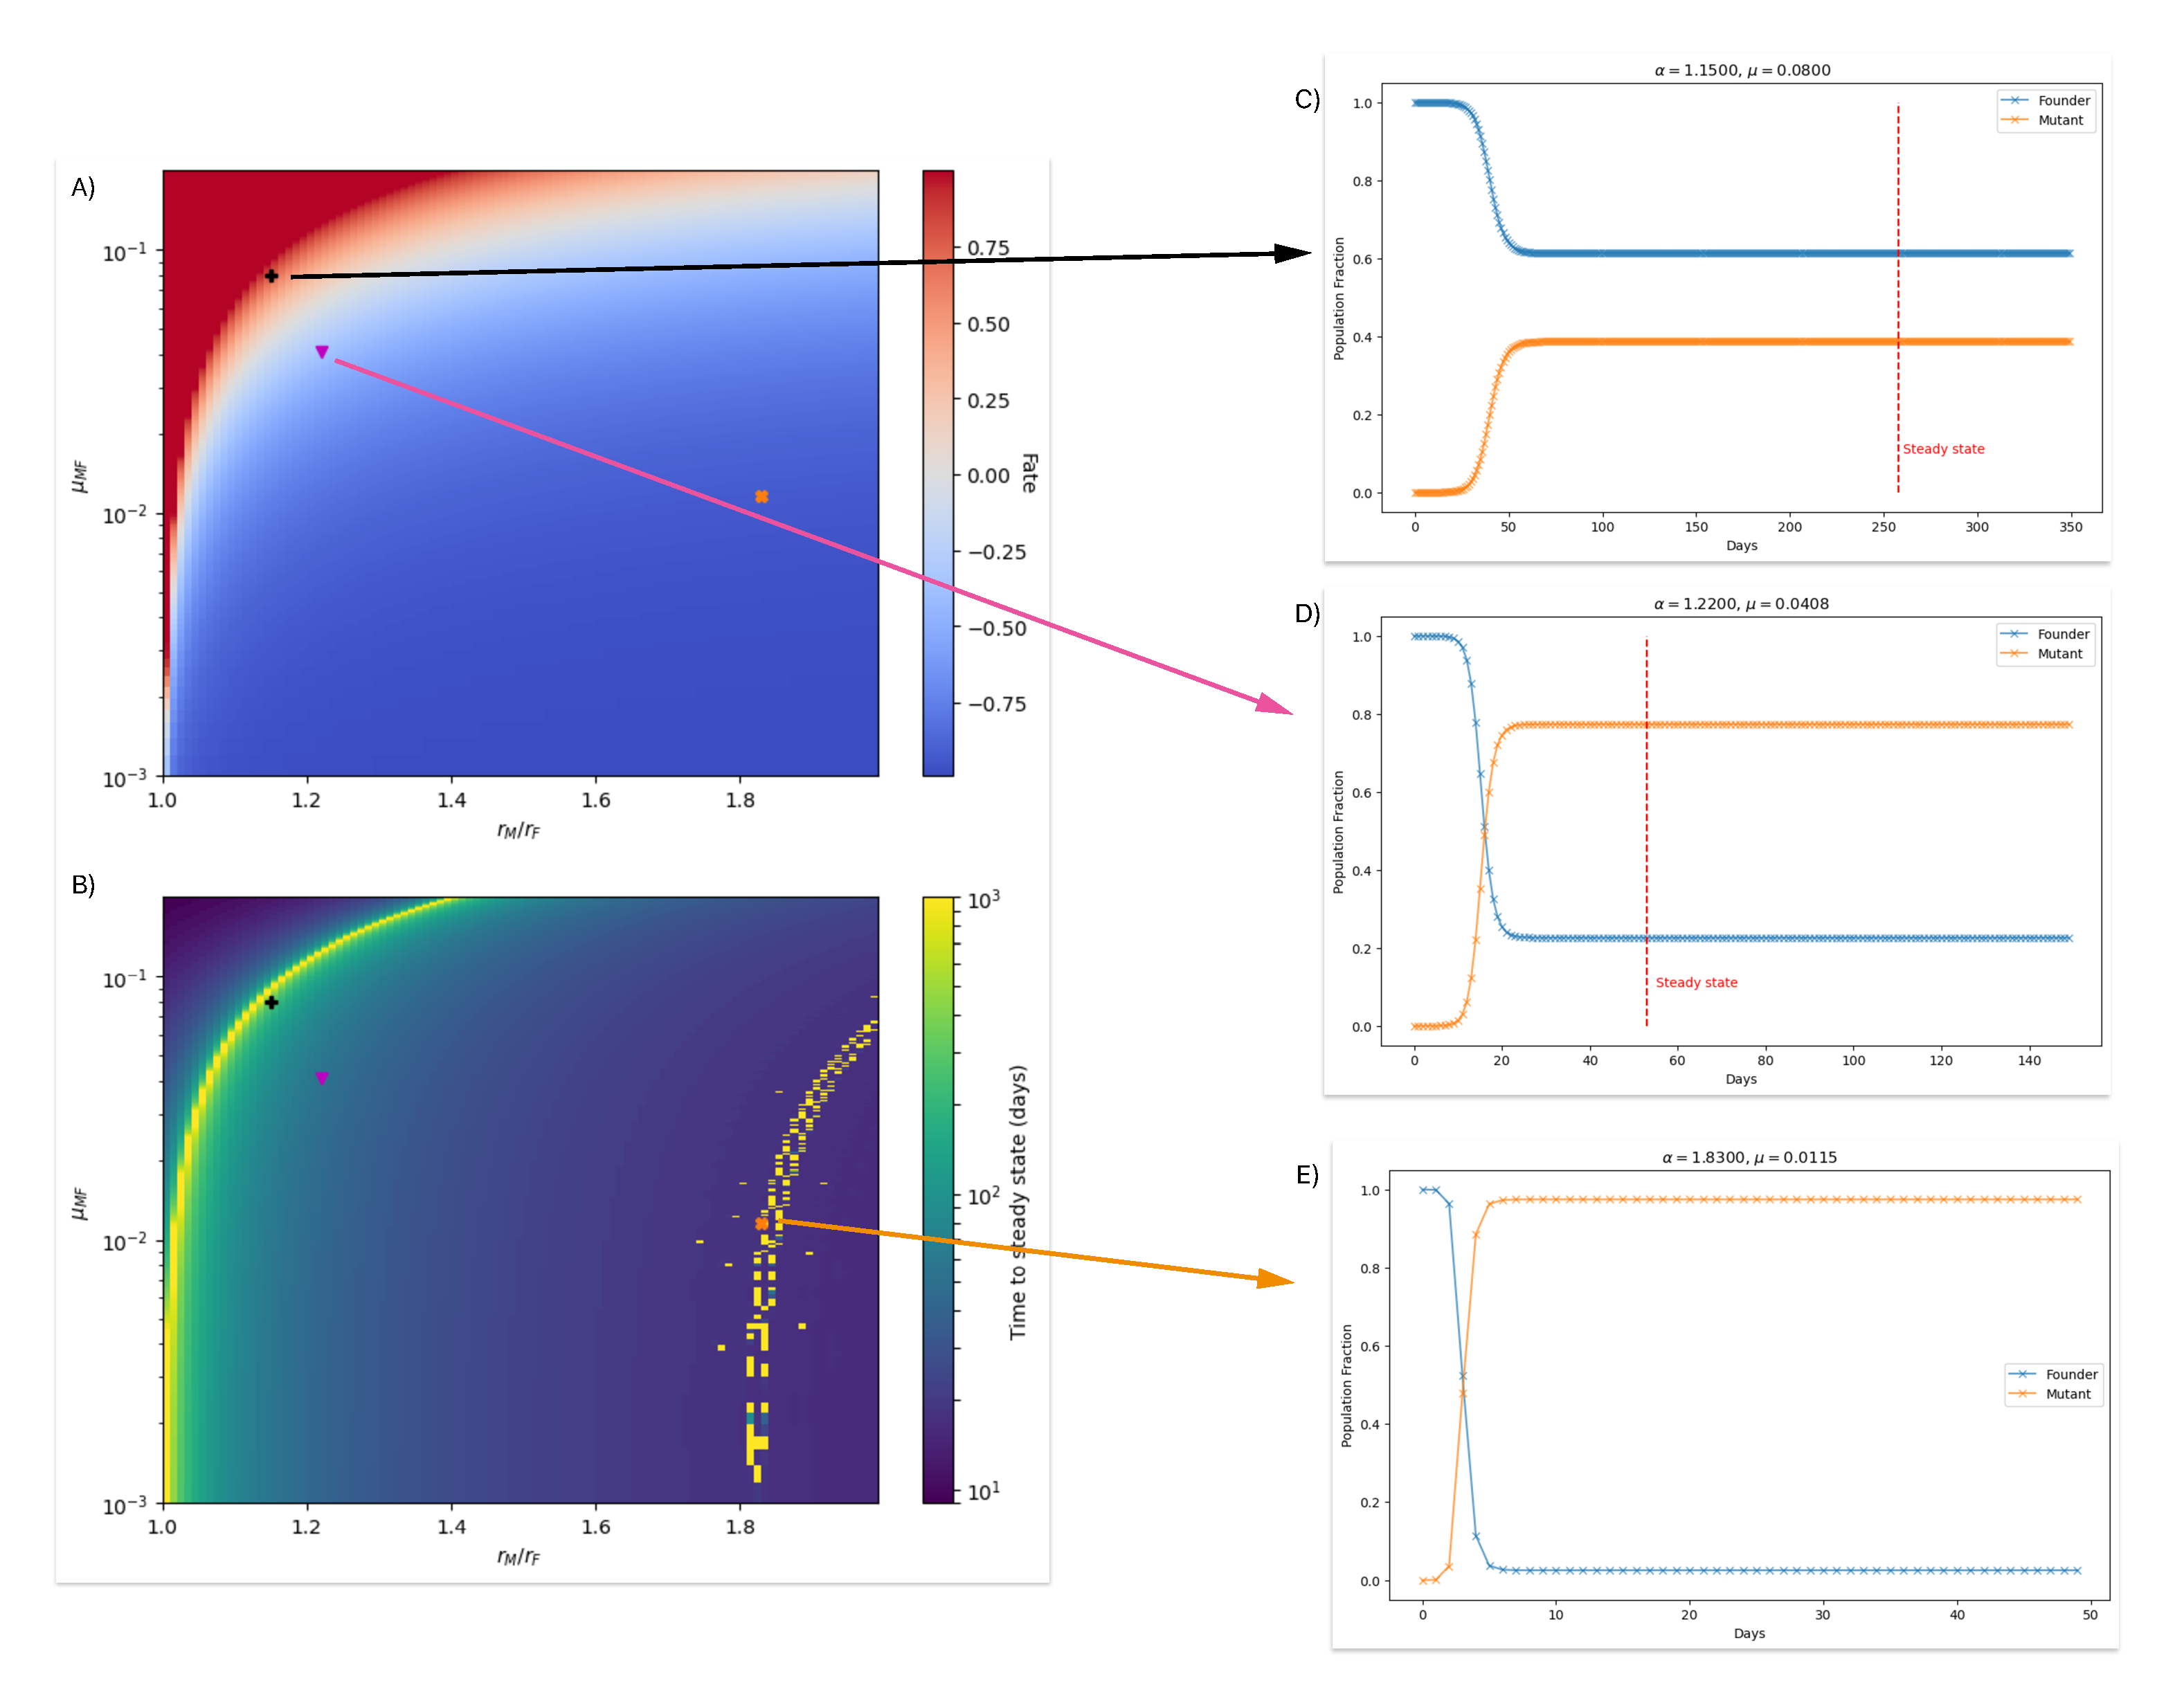
\includegraphics[scale=0.35]{big_plot_v2.pdf}
	\caption{Parameter space for the two state system. The left panel shows the difference between the bacterial abundance at the end of the experiment (top), and the time to reach the steady state (bottom). In the former, the intensity of the color indicates a higher abundance of founder (red) or mutant (blue). In the latter, the color grading represents the number of days to reach the steady state. The right panel shows the evolution of population fraction at the end of every day for areas of interest in the parameter space.}
	\label{fig:parameter_space_2st}
\end{figure}

The top panel in Figure \ref{fig:parameter_space_2st} displays the difference between the proportions of founder and mutant at the steady state. The red tones indicate a higher abundance of founder, whereas the blue tones higher abundance of mutants. The red areas support the intuition that a higher mutation loss rate combined with a low mutant replication rate result in a great abundance of founders, therefore there will be no coexistence of mutants and founders. A similar affirmation is true for 

All the lighter tones represent coexistence between founders and mutants, with a slight preference towards either population depending on the specific tone. We can see that coexistence is possible for most values of $\alpha$ but it only happens for $\mu_{MF}>10^{-2}$

In addition, we can relate the behavior in the population abundance with the time to steady state. The transition between bold and light red areas in panel A matches the yellower curve in panel B, implying that the transition between a state of coexistence to a state where the founder takes over the population causes the system to reach the steady state at a later time.

The right panel in Figure \ref{fig:parameter_space_2st} exemplifies of the evolution of the population fraction for different regions of the parameter space. C and D show two points at the coexisting region
The regions where one of the populations is dominant are characterized for small times to the steady state. These times get larger as we approach the regions where coexistence is possible. It is interesting to note as well, that this transition is seemingly smooth for the mutants and quite sharp for the founders.


%%%% Insert plot of the difference between populations

\section{Methods}

To solve the ODE systems, I used the \verb|numbalsoda| library in python

I used the MCMC implemented in python's \verb|emcee| package. This choice is purely based on familiarity with the package and the simplicity of its implementation

I used the ABC implementation in PyMC v5.10.4 with the \verb|sample_smc| function. I chosed 8 chains running on 4 cores of the M2 chip, the distance function is set to \verb|laplace| and the tolerance is $0.001$
The figure below shows the distribution of the chains for each parameter
\begin{figure}[H]
    \centering
    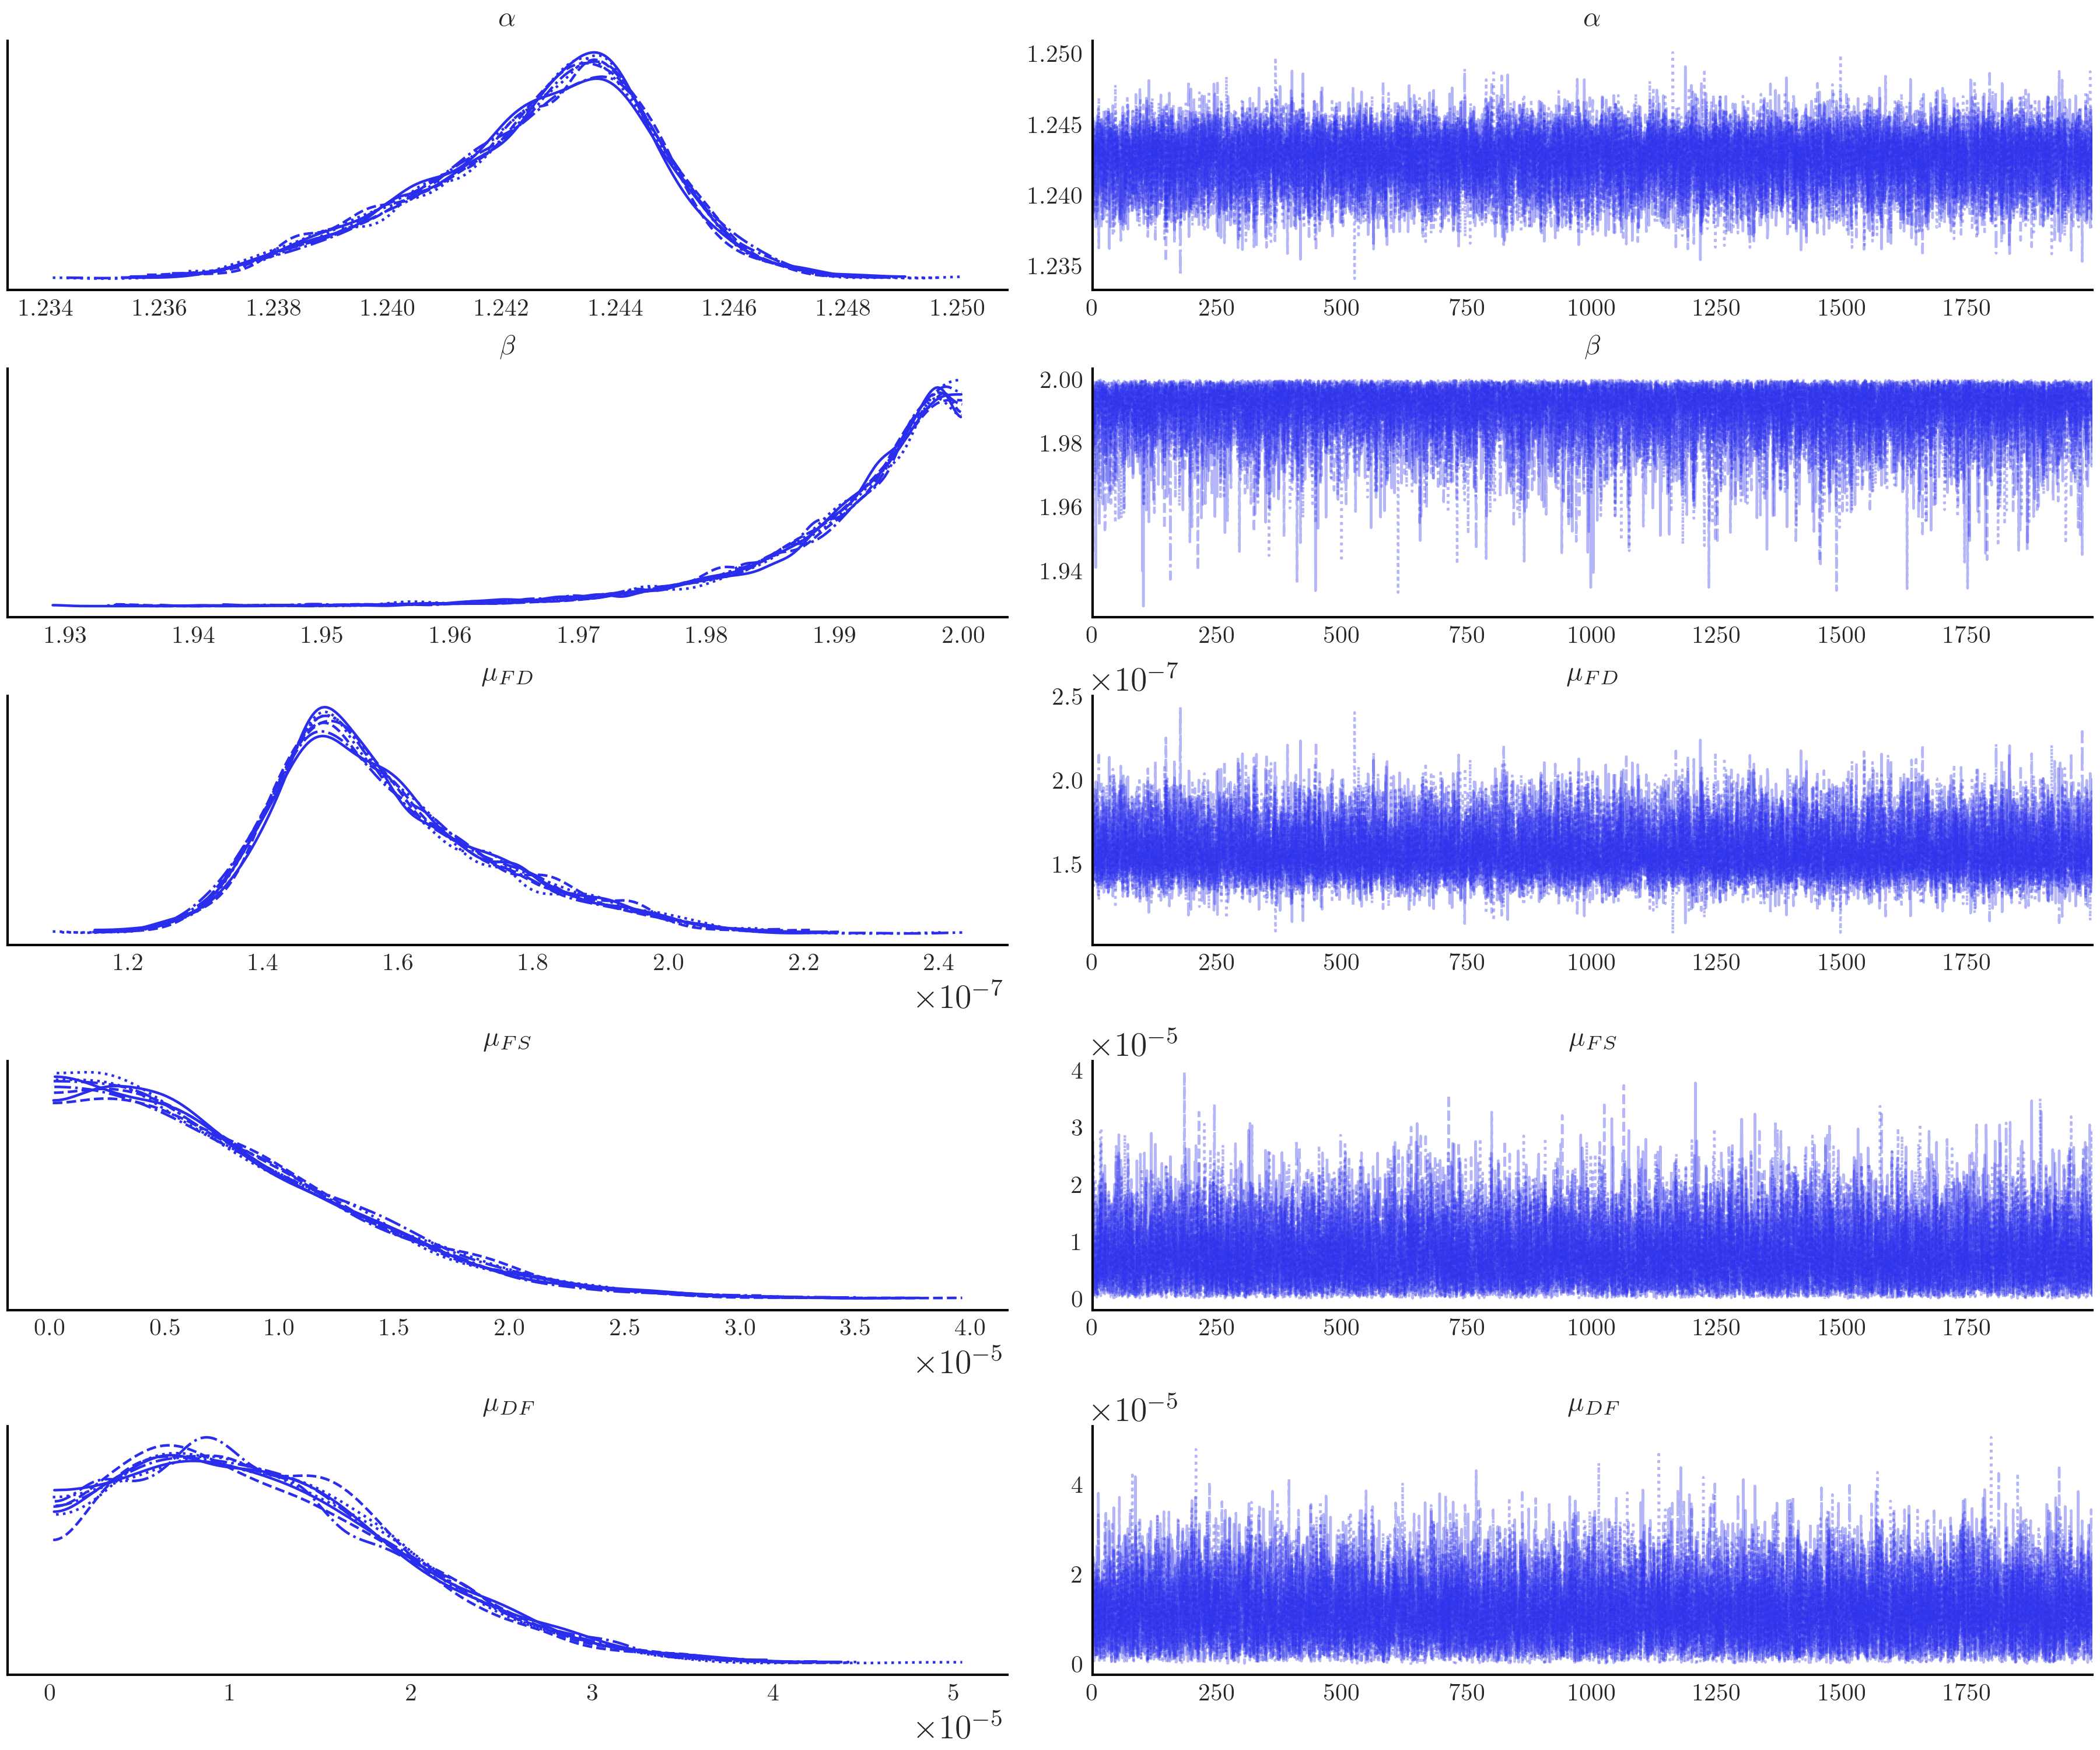
\includegraphics[width=1\linewidth]{plots/abc_3st_param_dist.png}
    \caption{Distribution of the chains for ABC results in Fig \ref{fig:posterior_abc_3st}}
    \label{fig:abc_3st_param_chains}
\end{figure}

\subsection{Determining convergence of the experiment}
To determine the convergence of the experiment we calculate the area under the population curves using the Simpson's method implementation in \verb|scipy.integrate.simpson|. In more detail, the procedure above is described by
\begin{equation}
	\vec{A}_n = \int_n \{F_n(t),M_n(t)\} \dd t,
\end{equation}

where $n$ represents a day in the experiment
\begin{equation}
	\|\vec{A}_n - \vec{A}_{n-1} \| < \epsilon
\end{equation}
where $\|\bullet\|$ is the euclidean distance. When this condition is satisfied for three consecutive days $(n, n+1, n+2)$ we say that the system has reached the steady state

\subsection{Pending tasks}
Here I want to summarize some tasks that are still pending without any particular order
\begin{itemize}
    \item Implement a measure for the goodness of fits from the parameters obtained by bayesian inference. So far I am only visually inspecting the results and there is no quantitative measurement of it
    \item So far I have been running all the inference algorithms for replicate 1 of the experimental data. Even though upon visual inspection all the replicates look indistinguishable, it is necessary to run the algorithms for the remaining replicates to compare the results and test the robustness of the predictions. Nonetheless, I don't expect the results to change significantly.
    \item We discussed at some point in the past weeks about the apparent symmetry of the equations. Running the experiment for the 2 state system interchanging all the parameters between Founder and Mutant will be useful to test that independence of the predictions
    \item I still need to address the time that it'll take the experiment to converge for different experimental conditions. Since so far I haven't found an analytical solution, the easiest way to do it will be to explore the parameter space using the knowledge gained from the bayesian inference results.
\end{itemize}

\ \newpage
\bibliographystyle{vancouver_modified.bst}
\bibliography{trna.bib}
%\printbibliography
\end{document}